% REMEMBER: You must not plagiarise anything in your report. Be extremely careful.

\documentclass{l4proj}

    
%
% put any additional packages here
%

\begin{document}

%====================================================================https://www.overleaf.com/project/61cdb5956bbdc463d8789a8f==========
%% METADATA
\title{A multiplayer bike-tracking game for phones}
\author{Hauwa Njidda}
\date{January 14, 2022}

\maketitle

%=========================================================
%% ABSTRACT
\begin{abstract}
    Bike tracking is now the common way of working out apps like Strava and MapMyRide which are both the most common cycling apps helps cyclists. Track bikes are meant for one thing and one thing only: track racing. They are not meant for road riding. Which now makes things fun for the bikers and for the ability of velodrome racers to balance their fixed-gear bikes on the track. In this project we look at applying a multiplayer based bike tracker, with the main features focusing on collaborative interaction. Implemented as an iOS application in the form of an app, we analyse the effectiveness of this approach to bike tracking through different usability evaluations. 
\end{abstract}

%==============================================================================

% EDUCATION REUSE CONSENT FORM
% If you consent to your project being shown to future students for educational purposes
% then insert your name and the date below to  sign the education use form that appears in the front of the document. 
% You must explicitly give consent if you wish to do so.
% If you sign, your project may be included in the Hall of Fame if it scores particularly highly.
%
% Please note that you are under no obligation to sign 
% this declaration, but doing so would help future students.
%
%\def\consentname {My Name} % your full name
%\def\consentdate {20 March 2018} % the date you agree
%
\educationalconsent


%==============================================================================
\tableofcontents

%==============================================================================
%% Notes on formatting
%==============================================================================
% The first page, abstract and table of contents are numbered using Roman numerals and are not
% included in the page count. 
%
% From now on pages are numbered
% using Arabic numerals. Therefore, immediately after the first call to \chapter we need the call
% \pagenumbering{arabic} and this should be called once only in the document. 
%
% The first Chapter should then be on page 1. You are allowed 40 pages for a 40 credit project and 20 pages for a 
% 20 credit report. This includes everything numbered in Arabic numerals (excluding front matter) up
% to but excluding the appendices and bibliography.
%
% You must not alter text size (it is currently 10pt) or alter margins or spacing.
%
%
%==================================================================================================================================
%
% IMPORTANT
% The chapter headings here are **suggestions**. You don't have to follow this model if
% it doesn't fit your project. Every project should have an introduction and conclusion,
% however. 
%
%==================================================================================================================================
\chapter{Introduction}
% reset page numbering. Don't remove this!
\pagenumbering{arabic} 


 
Cycling trackers have shown to be really handy in the cycling space, this has become very common everywhere since it is all remotely and easy to use. Modern cycling trackers can give insight into different aspects of a user's health ranging from generic cycling related feedback all the way to early identification of certain health issues \cite{boulos2021mobile}. 

\cite{dyck1976bicycling} , \cite{connollyevolution}Cycling history moves down to how it was first invented. A German baron named Karl von Drais made the first major development when he created a steerable, two-wheeled contraption in 1817. Known by many names, including the “velocipede,” “hobby-horse,” “draisine” and “running machine,” this early invention has made Drais widely acknowledged as the father of the bicycle. But the bicycle as we know it today evolved in the 19th century thanks to the work of several different inventors. Cycling is also used 

We believe that there is potential  to work on the human nature of activity tracking and introduce elements that have potential to inspire long term use. We look to apply a bike tracking that incorporates certain multiplayer cycling together, the implementation at its core looks to leverage the behavioural science of both game elements and habit formation.  

Additionally we look to evaluate the effectiveness and attitudes towards this gamified and social multiplayer activity tracking through a number of usability evaluations at different stages of the iterative design process.

\section{Guidance}


The efficacy of fitness tracking over longer periods raises questions over the merit of these trackers, with specific longevity issues with novice, shy and female users. As the popularity of fitness trackers continues to rise, the abandonment rates raise issues for the sustainability of traditional fitness trackers. The nature of traditional bike trackers are seeing novice users waste money on expensive equipment that they are unable to take full advantage of.


While popular traditional bike trackers such as Strava , MapMyRide and RideWithGPS, see \cite{lee2021strava}, \cite{bergman2016conflation} have looked to add some level of game elements, abandonment rates still remain high. The underlying approaches of these popular cycling trackers are that they do not have privacy control and the groups and not really welcoming. Also, not easy to new users to get to.

There is potential to introduce a future gamified experience with closure of not showing too many personal details and include or engaging with female and shy users. This can be done by following game design principles as well as the behavioural science behind habit formation, this approach would also account for different experience levels of users. Due to the inherently collaborative nature of games, it’s reasonable to assume gamification of certain features in the cycling tracking model could lead to a more collaborative / multiplayer experience with certain privacy. In this project we attempt to add certain multiplayer aspects to the traditional cycling model.

\section{Writing guidance}
\subsection{Who is the reader?}

This is the key question for any writing. Your reader:

\begin{itemize}
    \item
    is a trained computer scientist: \emph{don't explain basics}.
    \item
    has limited time: \emph{keep on topic}.
    \item
    has no idea why anyone would want to do this: \emph{motivate clearly}
    \item
    might not know \emph{anything} about your project in particular:
    \emph{explain your project}.
    \item
    but might know precise details and check them: \emph{be precise and
    strive for accuracy.}
    \item
    doesn't know or care about you: \emph{personal discussions are
    irrelevant}.
\end{itemize}

Remember, you will be marked by your supervisor and one or more members
of staff. You might also have your project read by a prize-awarding
committee or possibly a future employer. Bear that in mind.

\subsection{References and style guides}
There are many style guides on good English writing. You don't need to
read these, but they will improve how you write.

\begin{itemize}
    \item
    \emph{How to write a great research paper} \cite{Pey17} (\textbf{recommended}, even though you aren't writing a research paper)
    \item
    \emph{How to Write with Style} \cite{Von80}. Short and easy to read. Available online.
    \item
    \emph{Style: The Basics of Clarity and Grace} \cite{Wil09} A very popular modern English style guide.
    \item
    \emph{Politics and the English Language} \cite{Orw68}  A famous essay on effective, clear writing in English.
    \item
    \emph{The Elements of Style} \cite{StrWhi07} Outdated, and American, but a classic.
    \item
    \emph{The Sense of Style} \cite{Pin15} Excellent, though quite in-depth.
\end{itemize}

\subsubsection{Citation styles}

\begin{itemize}
\item If you are referring to a reference as a noun, then cite it as: ``\citet{Orw68} discusses the role of language in political thought.''
\item If you are referring implicitly to references, use: ``There are many good books on writing \citep{Orw68, Wil09, Pin15}.''
\end{itemize}
\subsection{Plagiarism warning}

\begin{highlight_title}{WARNING}
    
    If you include material from other sources without full and correct attribution, you are commiting plagiarism. The penalties for plagiarism are severe.
    Quote any included text and cite it correctly. Cite all images, figures, etc. clearly in the caption of the figure.
\end{highlight_title}


%==================================================================================================================================
\chapter{Background}

 
Before getting into the product, it is always, if not necessary to research solutions that already exist. This will help develop a better experience that allows to stand out from the rest. For each competitor, we focused on what was excellent and what could be improved. 

- APP1 = STRAVA

Likes = Its easy and free to track your running
             Can help you discover running routes
 
Dislikes = Lack of Privacy
                  Fear of judgement

- APP2 = MapMyRide

Likes = Connect to other apps and certain devices 
             Clean modern design
             Made with unlimited mapped routes
             Connect with social media
 
Dislikes = Live tracking only available in paid version
                 Ads on the free version


- APP3 = RideWithGPS

Likes = Detailed routes straight on the map
             Search functionality for routes in your area
             Tracks cycled miles with certain gear
 
Dislikes = Split time available in paid versions
                  Difficult to handle for some cyclists

All these adds up to be able to solve the problem that is facing in these. Adding up other flaws will help me make better decisions for my cycling app.



\section{Guidance}
\section{Bike Tracking}

Bike tracking is a method of tracking activity through software applications. It has become really common especially in the modern world of cycling. A velodrome is an arena for track cycling. Modern velodromes feature steeply banked oval tracks, consisting of two 180-degree circular bends connected by two straights. Ever since in the traditional time it has been a means of entertainment.


\subsection{Traditional Bike Trackers}
\label{traditionalBike}
In the beginning, back in the 1890s, Six Day races were just that, six days or 144 hours of continuous racing, with the rider who completed most laps of the velodrome track winning.\cite{oke2015tracking}
Eventually, riders were put together in teams (usually a pair, but occasionally teams of three), with only one rider in the race at the same time, and exchanges being done by hand-slinging the teammate into the race.
This was first practised in New York’s Madison Square Garden in 1899, and the new discipline acquired the name ‘Madison’ from that venue.
During the heyday of the sport, from the 1950s to the 1980s, there were 30 or more Six Day races each year. Today, only seven remain – London, Gent, Rotterdam, Bremen, Berlin, and Copenhagen - as well as the summer Six Day event in Fiorenzuola.
Three of these - London, Berlin and Copenhagen - are part of the British-owned Six Day Series that started in the 2016/2017 track season.For this year, the Six Day Series added four new three-day events in Melbourne, Hong Kong, Manchester and Brisbane, in an effort to open up new markets.
With input from riders and officials at Six Day Berlin, I analyse the Six Day Series concept meant to rejuvenate six day racing. 

It was more common that men cycle more than women since in the beginning. It has always been that way and that was later changed or drafted to having women to cycle more. 

\cite{sanders2019intensity} Like base on a study by Dajo Sanders, a sport science who is at Strirlinh Univeristy. He research about the and studied the race data for 20 men and 10 women, all where professional cyclists with the World Tour Professional Cycling team. Pro cyclists, needless to say, spend a lot of time cycling, typically covering about 15,000 to 22,000 miles a year for men, and 8,000 to 11,000 miles for women, according to the researchers.

 A lot of that time is spent racing: up to 100 days a year for men and 65 days a year for women. For most of those racing days, the team’s science crew collected three complementary pieces of data: heart rate, which gives a sense of physiological strain; power output, which gives an impartial reading how hard the rider is pedaling; and perceived exertion, which gives a subjective take on how hard the race was.
 In total, over a four-year period, the team collected data on 3,640 days of racing by the 30 riders in the study.The average distance of a race day for the men was 114 miles, which took four hours and 45 minutes; for women it was 72 miles, which took three hours and 14 minutes.
 
 \cite{van2019training}In another study between 2000 and 2019, more men (63.1 of male participants and 52.2 of female participants) competed in 24 h races. Overall, women cannot keep up with the cycling with men which is intimidating for women and a discouragement.




\subsection{Facilitating health behaviour change}\label{healthbehaviourchange}

As we have discussed the default of traditional bike history trackers, it is imperative that we also discuss how to facilitate health behaviour change for long term efficacy of bike trackers. 

\cite{van2019training} Wu Sum Nathan Roberts suggest that there is little evidence to suggest that these traditional trackers and wearable facilitate long term health behavioural change. \cite{gidaris2019surveillance} Ledger McCaffrey  argue that while activity trackers provide the utility to users they do not incite change,  and while \cite{lemos2019move} Ledger McCaffrey focus on the long term engagement of wearable devices majority of their analysis filters through to the software products that accompany them. \cite{lemos2019move} Ledger McCaffrey go on to identify three main behavioural science factors that effect the long term engagement of fitness trackers, these three factors are: habit formation, social motivation and finally goal reinforcement. 

In addition to health behaviour, enhancing social connectedness can significantly improve quality of life, boost health and well-being, elevate mood and happiness, increase longevity, and even enhance cognitive and physical performance. Enhancing social connectedness can lengthen telomeres, ensuring that they continue to function effectively. During cell division, healthy telomeres prevent fraying—they act like “aglets,” the plastic caps on the ends of shoelaces. After numerous cell divisions, though, telomeres may become too short to protect our chromosomes, allowing cells to wither and die. Cellular death can increase the chances for chronic disease to develop, reducing life expectancy \cite{greider1996telomeres}

The final behavioral science studies the way that emotions, the environment and social factors influence our decisions. Behavioral science is particularly interested in how heuristics, biases and framing can lead us to make “irrational” decisions. Behavioral science borrows heavily from the methodologies developed in the social sciences, mainly running experiments using randomized control trials that allow us to make causal inferences about specific mechanisms that drive human behavior.\cite{wu2016fitness} suggest that users need to experience a feeling of progress to achieve sustained engagement, the author's go on to advocate that users require objective feedback about progress and their specific milestones. An important aspect to not just achieving sustained engagement but fitness as a whole is the user momentum, giving user's the right feedback enables them to continue and experience regular progress, gaining momentum in the mean time. The most common implementation for goal reinforcement in modern fitness trackers is through cues such as haptic feedback or push notifications for wearables and applications respectively. 




%==================================================================================================================================
\chapter{Analysis/Requirements}


Cycling has mostly been populated by men and little to no space for women. Since in the traditional times it has always been like that. Also, lack of privacy is key since in the modern days it has been a trouble for users and the fear of it has increased  very deeply. The analysis of more than 20,000 apps found that inadequate privacy disclosures for many of them prevented users from making informed choices about their data. One third could collect user email addresses and many more transmitted data to third parties such as advertisers. \cite{mayer2012third}. With all that this will be broken down the steps taken to solve the problems. 

\section{Guidance}

This chapters looks to outline the requirements of the project as a whole. As the project itself follows an iterative design process, this chapter will be split into different iterations. This will allow for the distinction of requirements at different phases of the development life cycle.

\section{Iteration One}


The main aspect of part one was concept generation ,which is further discussed in more detail \textbf{Section \ref{conceptGeneration}}.
To bring up idea such will solves the traditional cycling, it was important to do more research into the long term engagement of the tracking app. 

From researching the other similar cycling trackers and general considerations for what type of features would be expected in the cycling tracker, the main requirements were: Information display, group players, awards by badges, competitions, tracking functionality. To add up and visualise this requirement for this design choice the first step was to implement these as a rough sketch then as a paper prototype. The rough sketch helped in showing more varities then after choosing the suitable. The paper prototype displays the implementation  of this concept and these are discussed further in \textbf{Section \ref{conceptGeneration}}.

The final stage of this iteration was to have a user persona and user stories,  Since we use bicycle for so many things from use as delivery to use as sports. It was best to have a user persona.
A user persona is a semi-fictional character based on your current (or ideal) customer. Personas can be created by talking to users and segmenting by various demographic and psychographics data to improve your product marketing.The User stories shows the journey of the target users




\section{Iteration Two}
Iteration two progressing from the paper prototype to wireframes, while working on the Wireframe it was also possible to introduce a new concept as part of the concept generation phase. This shows for the requirement for the second iteration was as follows: convert the paper prototype to wireframes, identify new ideas on the current design , and run some form of evaluation on these wireframes. It includes the think-aloud evaluation run on these are discussed in \textbf{Section \ref{ThinkAloud}}.



\section{Iteration Three}\label{requirementsIterationThree}


Iteration Three consisted of mainly moving the paper prototype to more opened prototype, user journey of using the prototype and testing the prototype. 
This shows the prototype with Refacturing UI and Colour Palette. With the a guide to Know About the Types of Color Palette and Creating a UI Color Palette for Best Results. Several types of colour palettes, which are 
- Monochromatic Palette which are considered or have different tint , shades and tones. \textbf{Section \ref{Monochromatic}}.



- Analogous Color Palette which as three consecutive colors on a color wheel make up your analogous color palette. 


- Complementary Colors which most designers choose two colors along with their tints, shades, and hues that complement each other or add to each other's presence.



- Triadic Color Palette this is the easiest to do because when you want to add three different shades to your design.


- Split Complementary this is where things start to get a bit intense. In a split complementary UI palette of colors, you have to play with three colors and, yes, all of their different variants across the spectrum.



- Tetradic Color Palette The tetradic UI color palette is a combination of four different colors, or we can say two complementary pairs. Also, the two colors on either side of the color wheel should be alternates, but that will naturally occur when you choose two complementary color. 


Moving into the buttons and the icons. This is really important for users to identify which button is for what. Buttons actions are not fully about the style although users do get use to the styling. The call to action which depends on the situation this will attract the user to wither register, signup, logout etc. The common button styles which was all have consistent style  implemented are the 

- Solid button this was mostly common for the direct call to action. like the login in and register button 

- Rounded button whose edges are set to the max rounded border-radius.

- icon button have no label and are only an icon. Because they don’t have a label, they save a lot of space in an interface.

Base of The Psychology of Colours, it’s a well-known fact that colors can provoke emotions, every color evokes a different feeling or mood with people and, therefore, results in a different reaction when seeing the color (of course, it is relative as different cultures perceive color differently). \textbf{Figure \ref{fig:PsychologyofColours}}.
 





\begin{figure}
    \centering
     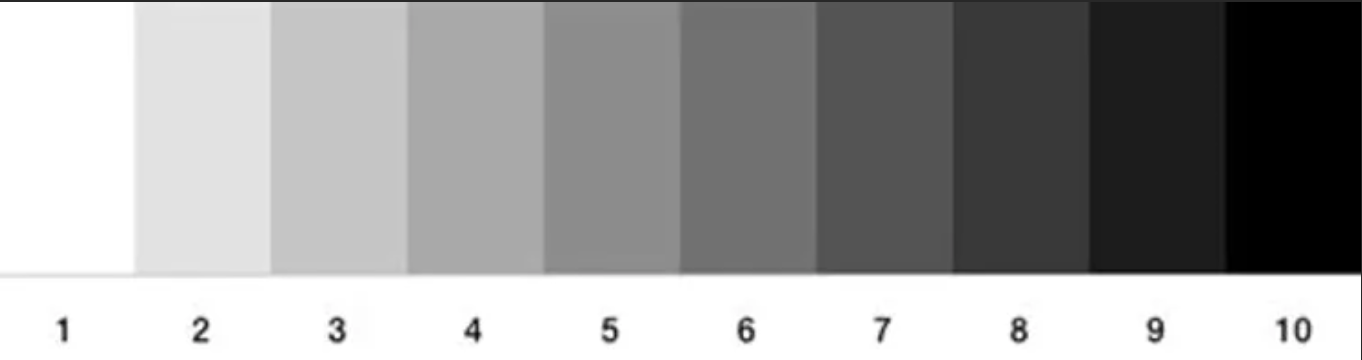
\includegraphics[width=1\textwidth]{images/mono1.png}
     \caption{Monochromatic}
    \label{fig:Monochromatic}
\end{figure}





\section{Iteration Four}\label{requirementsIterationThree}

The final iteration consisted mainly of software development and usability testing. The requirements of this iteration can be split into different phases, with the initial phases consisting of mainly software development and the latter phases with usability testing.After the first week of testing feedback was gathered with new feature requests being identified.These new features were done during the time frame. A final requirement of the software development life-cycle and the iterative design process was to again gather feedback based on the final phase of usability testing with the new features implemented. It was decided the most efficient form of user evaluations would be in the form of interviews, these are discussed further in \textbf{Section \ref{HeuristicEvaluation}}.


\begin{figure}
    \centering
     
\includegraphics[width=1\textwidth]{images/mono.png}
     \caption{Monochromatic}
    \label{fig:Monochromatic}
\end{figure}

\begin{figure}
    \centering
     
\includegraphics[width=1\textwidth]{images/090.png}
     \caption{Psychology of Colours}
    \label{fig:PsychologyofColours}
\end{figure}

\subsection{Functional Requirements} \label{functionalRequirements}

Functional requirements are comprised of both product features and user requirements.Some examples of functional requirements include: Specifications of what the system must do,Business rules that must be met, Steps that the system must take in authentication, Details of what must be tracked in the system. 
\subsubsection{Must Have}
These are the features that are really essential to a working cycling tracker, these are crucial to the application and they help with the evaluations and testing possible. The Must Have features are:  

Activity tracking: This is one of the most important part of cycling tracking. 
cyclometer an instrument for measuring circular arcs it is attached to a bicycle for measuring the distance it travels. Tried using similar feature in the tracking app.

Real-time Database: This enable real-time data collected by the activity. To enable real-time data communication a fast back-end database is required,  requires a serverless approach for both up-to-date activity tracking and the battle mechanics, a real-time database that seamlessly integrates into the iOS application is a core requirement.

Game elements: game elements and mechanics are important for driving the social and enjoyable side of the bike tracking app. There are features included in games that help immerse us in the play experience. If the game is being designed for commercial purposes, the sole aim is to come up with game mechanics that are fun. But when trying to design effective learning games, game mechanics and game elements that are utilized have to complement the learning goals. There are so many game mechanics that can be utilized for this design. Game plays a good role with the engagement of people and socializing with people with regards to the type of users the app is.



Race Search mechanics: To incorporate external consistency it would be ideal to implement an automated search. Most existing games that have some form of matchmaking implement a skills based matchmaking approach. To incorporate this we could look to match based on levels and ranks, however due to the planned number of participants this approach may be infeasible as getting two users searching simultaneously is highly unlikely. This feature is also time consuming and as it is not identified as a core component suitable alternatives may need to be identified. 


\subsection{Non-Functional Requirements}

Non functional requirements are focused on how the system goes about delivering a specific function. At first glance they might be seen as less important than functional requirements but both have a part to play in a good system. Non functional requirements do not have an impact on the functionality of the system but they do impact on how it will perform 

\subsubsection{Must Have}\label{nonfuncmusthave}
These features or properties are not core to the base functionality and the application should be able to function without them, but as we look to develop a user experience that accommodates the longevity of the application they have been included. The Must Have components are: 

Stylish User-Interface design: As the user interface can greatly affect the feelings towards an application, it is important that the interface conforms to the expectations of a modern and relatively stylish application. There are a number of ways to achieve this, potentially by following user-interface guidelines such as Apple's Human Interface Guidelines, however for this project we have approached a graphic designer to help create basic wireframe designs to base the final design on. These final designs are tweaked to accommodate all the expected functionality and are showcased in \textbf{Section \ref{final design}}. 

\subsection{Usability Evaluation Feedback} \label{usabilityevaluationfeedback}

As discussed previously, the final iteration was split into two phases. The second phase consisted of identifying new potential features based on user feedback after the first week of usability testing. As we look to follow the iterative design process it was important to incorporate this stage into the life-cycle, allowing for refinement of the product and identifying shortfalls. The feedback was gathered using an online survey with a combination of closed-ended and open-ended questions. From there potential features were identified such as more detailed data displayed, leaderboards, Scores and the ability to view the progress of other groups. 




%==================================================================================================================================
\chapter{Design}


\section{Concept Generation} \label{conceptGeneration}

To create a system that would incorporate collaborative features it was important to follow a structured framework for the concept generation. This framework facilitated exploring different collaborative \& competitive features, as well evaluating them swiftly to determine which would be effective or not. As is the nature of the design funnel and an iterative design process, this project was split into iterations, moving from low-fidelity paper-prototypes and early-stage wireframes, to higher-fidelity wireframes and prototypes. 

As outlined in \textbf{Section \ref{traditionalBike}}, traditional fitness trackers lack social elements and are individualistic in their approaches. With these considerations it was important to generate concepts that exhibited collaborative elements that stimulated a multiplayer environment. Elements and game mechanics such as leader boards, levels and group competitions were all considered as key components in designing a multiplayer activity tracker. The initial phase of design overlaps with iteration one. The early ideas that were translated into paper prototypes were a range of STRAVA tracker, MapMyRide and an exploration of more group bike  trackers.Continuing inline with the design funnel heuristic evaluations were performed on these paper prototypes, and are discussed in \textbf{section \ref{HeuristicEvaluation}}. From the results of these evaluations, and based on general analysis and research into traditional bike tracking. 

Iteration two presented the opportunity to expand the design space, with the identification of the shortfalls of the previous paper-prototypes, a new concept the Activity pet was introduced. This is essentially a multiplayer battle game fuelled by quests and activity. Iteration two also presented the opportunity to flesh-out the basic paper prototypes of the ideas that survived the controlled convergence of the first iteration and the new concepts introduced in iteration two. 
 For this iteration Think-Aloud evaluations were run with the use of the biking apps these are discussed in \textbf{Section \ref{ThinkAloud}}.


\subsection{User Persona}
Since we use bicycle for so many things from use as delivery to use as sports. It was best to have a user persona.
A user persona is a semi-fictional character based on your current (or ideal) customer. Personas can be created by talking to users and segmenting by various demographic and psychographic data to improve your product marketing. as seen in \textbf{Figure \ref{fig:persona}}. This persona personality is shy, being an introvert. She has little to no time for herself and what she loves. So, with the right app for her personality. This was the type of target to the work. Although, the work comprises of other factors. We made it for all in a friendly yet comfortable app for users like Jasmine. 

\begin{figure}
    \centering
     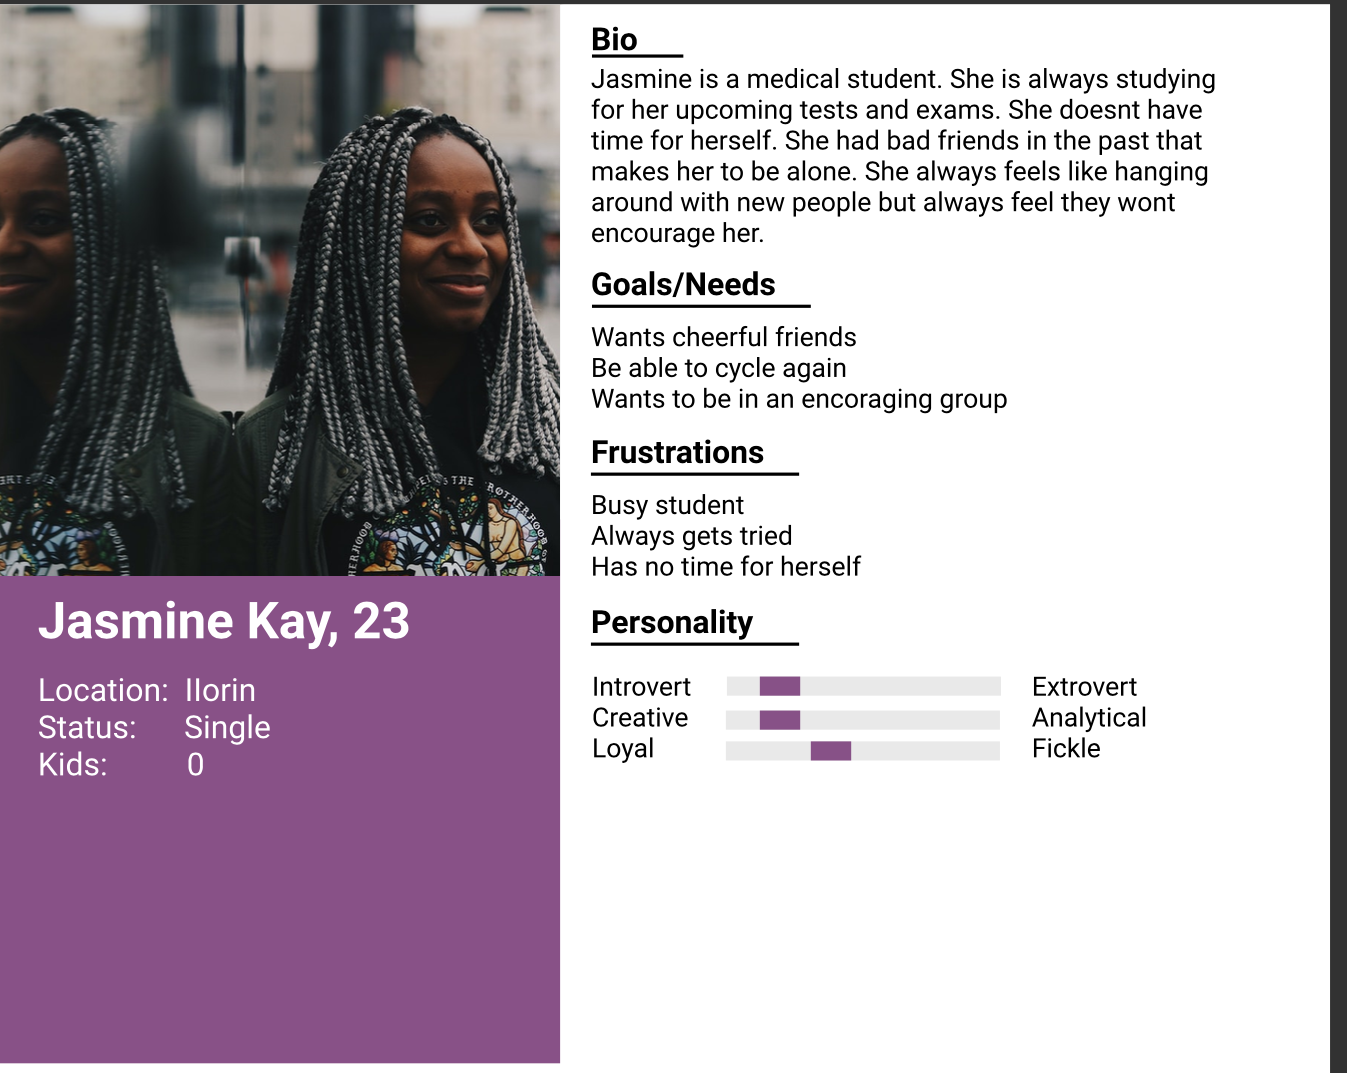
\includegraphics[width=1\textwidth]{images/Persona.png}
     \caption{Persona}
    \label{fig:persona}
\end{figure}
\vspace{3 cm }
\subsection{Storyboard}
After creating the user persona, it down to the type of user. Later,  created the user story behind this user persona. What will this person do. Graphic organizer in the form of illustrations or images displayed in sequence for the purpose of pre-visualizing a story. This makes it easier on what the app will be and look like when being used on the actual user persona 

Firstly, the idea of having the storyboard on a paper seemed straight forward  as seen in \textbf{Figure \ref{fig:paperstroyboard}}
 but it was later moved to a digital storyboard this shows the clear scenario with where and how it takes place.  \textbf{Figure \ref{fig:digitalstroyboard}}
Story:
Jasmine joined wheeler app so that she can be motivated to workout more. After joining a group she had a specific time to start the race and location. She was a bit nervous with the new faces. When the race was about to end, the app made them to move faster. At the end of the race the results where shown. She noticed that it was id given to all individuals in the group this helped them protect their identity and this reduced her parnoiar. Also, the app showed the weakest cyclist and we had to encourage the individual to ride more so that they can achieve the next rank together.

\begin{figure}
    \centering
     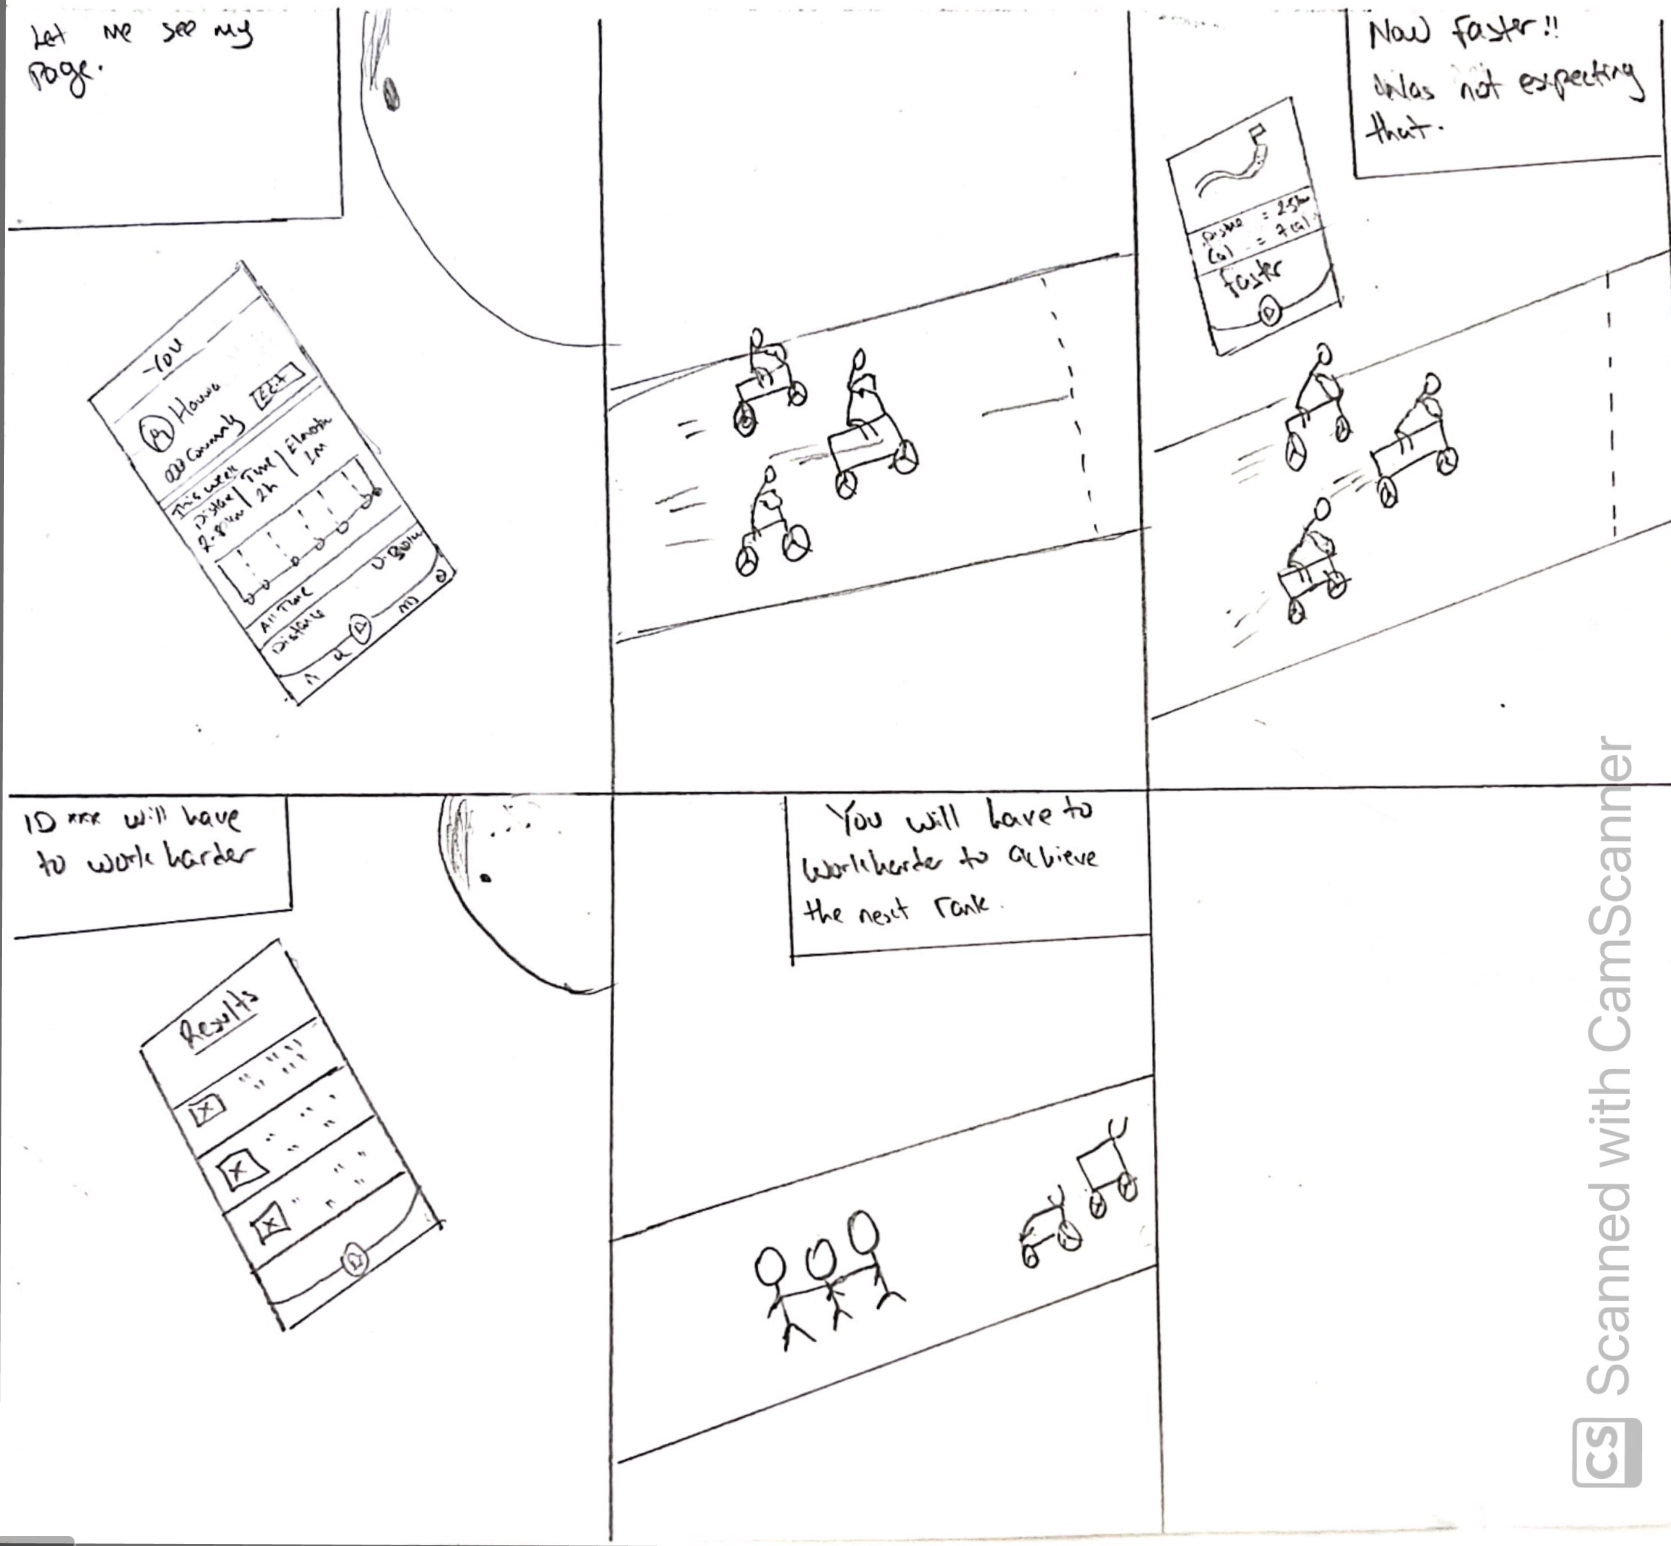
\includegraphics[width=.7\textwidth]{images/paper stroy.png}
     \caption{Paper Paper stroyboard}
    \label{fig:paperstroyboard}
\end{figure}

\subsection{Paper Prototypes}

Paper prototypes were used for the initial concept generation because they are notable for being easy-to-implement prototypes. For iteration one this was ideal as it was an effortless way of visualizing ideas and evaluating their potential. To provide a better visual depiction for the sake of this project all paper prototypes have been converted to wireframes, however it is important to note that this is solely for reporting purposes and actual paper prototypes were used in practice.

\begin{figure}
    \centering
     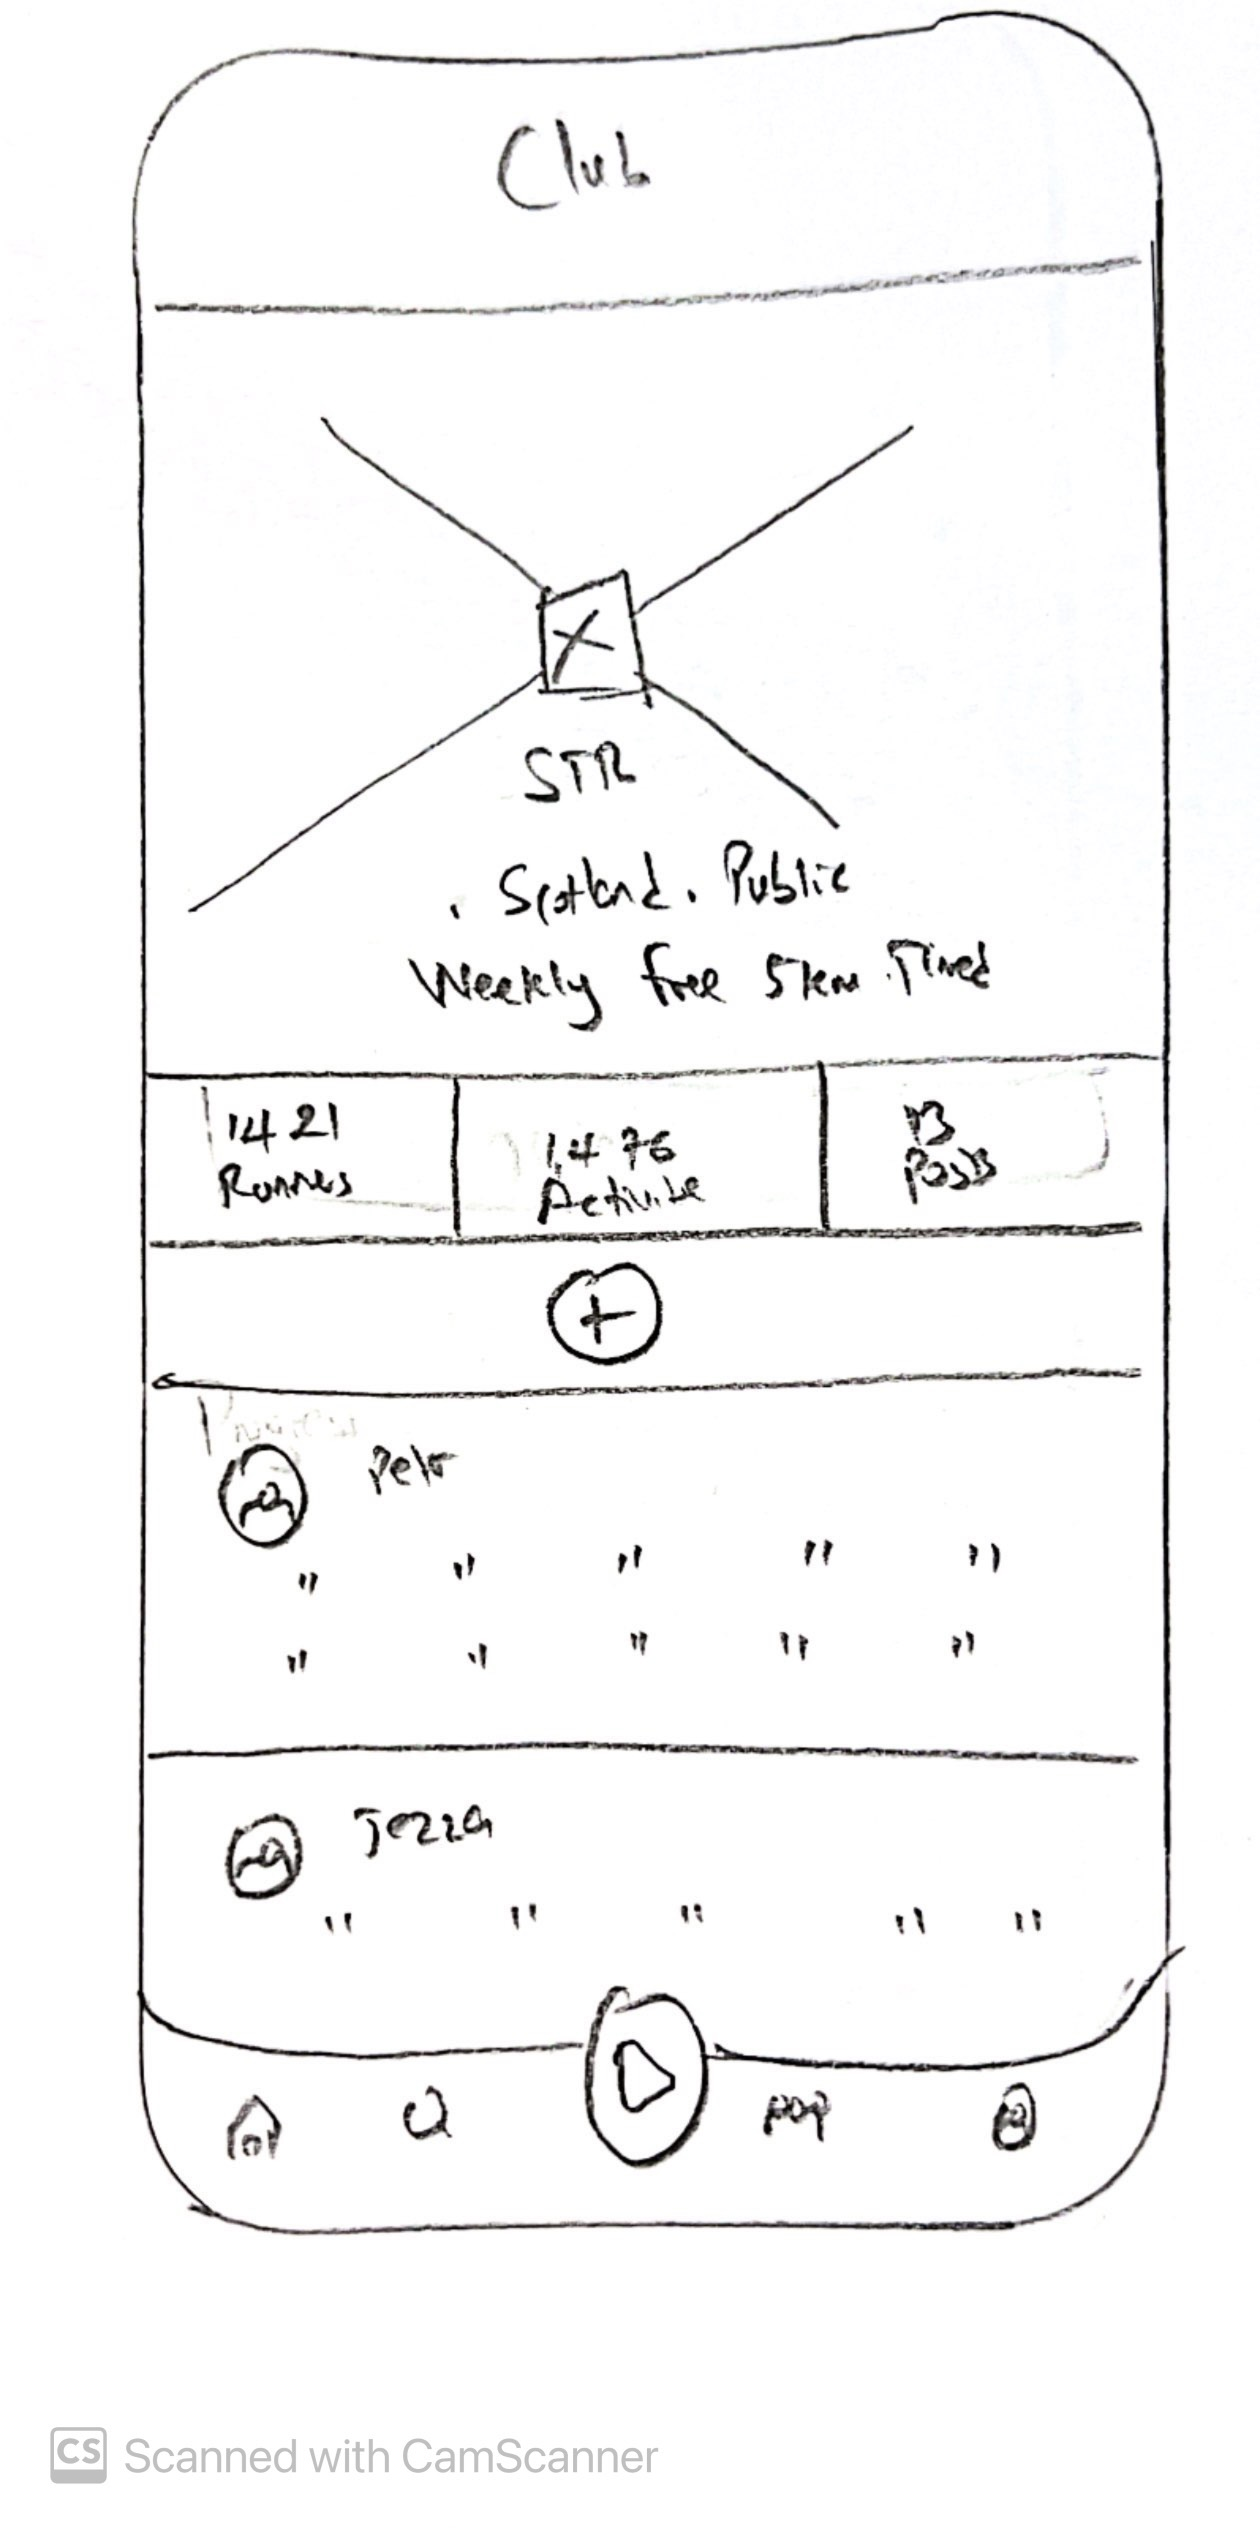
\includegraphics[width=.3\textwidth]{images/IMG_7031.JPG}
     \caption{Paper Prototype}
    \label{fig:my_label}
\end{figure}
%==================================================================================================================================








\begin{figure}
 \centering
 \begin{minipage}[b]{0.55\textwidth}
  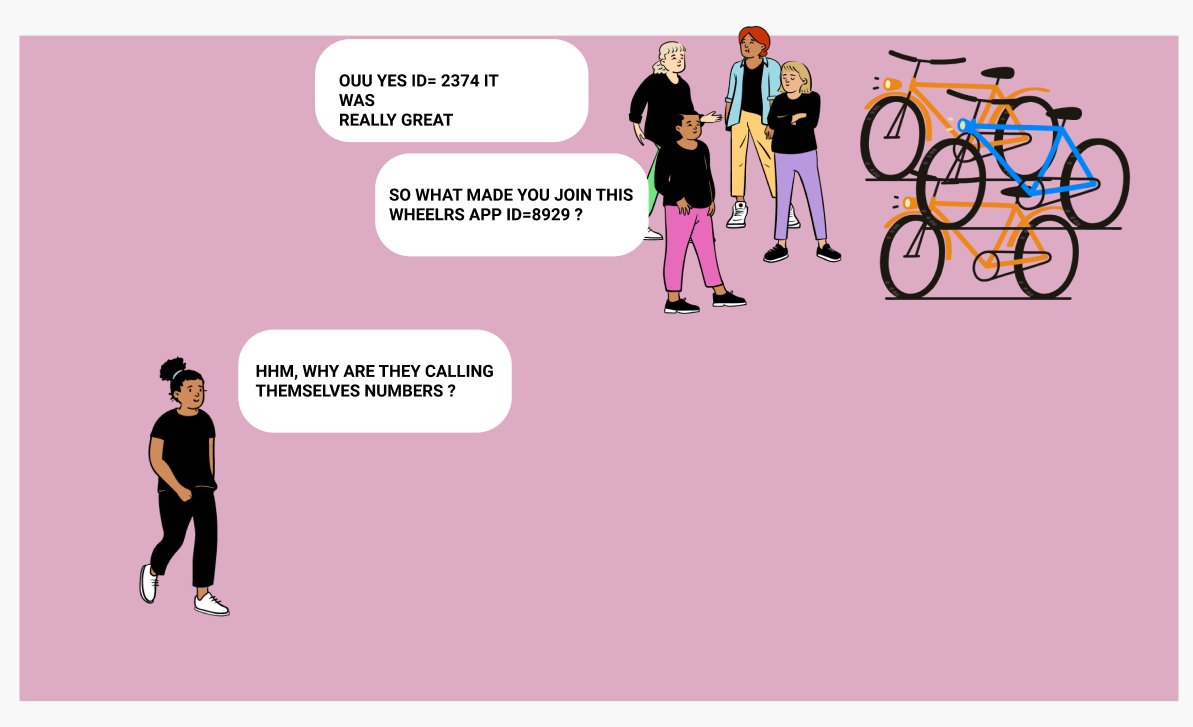
\includegraphics[width=1\textwidth]{images/1.png}
  \caption{ 1 Digital storyboard}
 \end{minipage}%
 \begin{minipage}[b]{0.55\textwidth}
  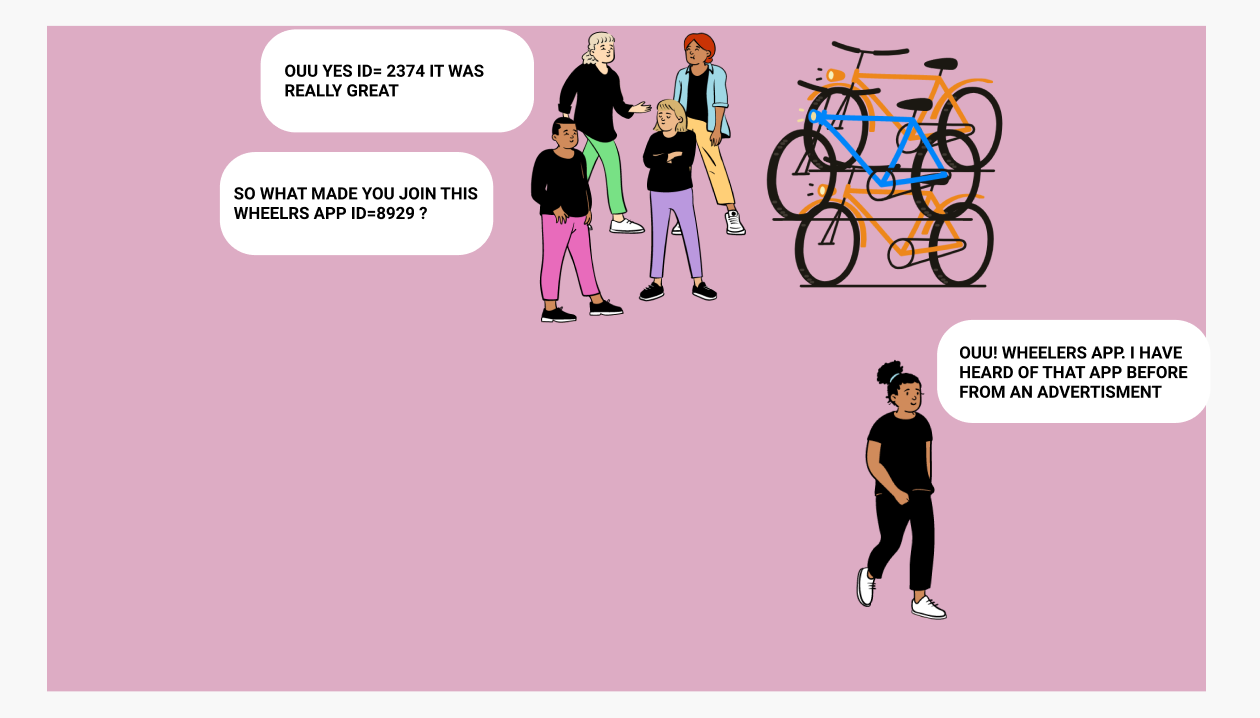
\includegraphics[width=1\textwidth]{images/2.png}
  \caption{2 Digital storyboard}
 \end{minipage}
\end{figure}

\begin{figure}
 \centering
 \begin{minipage}[b]{0.55\textwidth}
  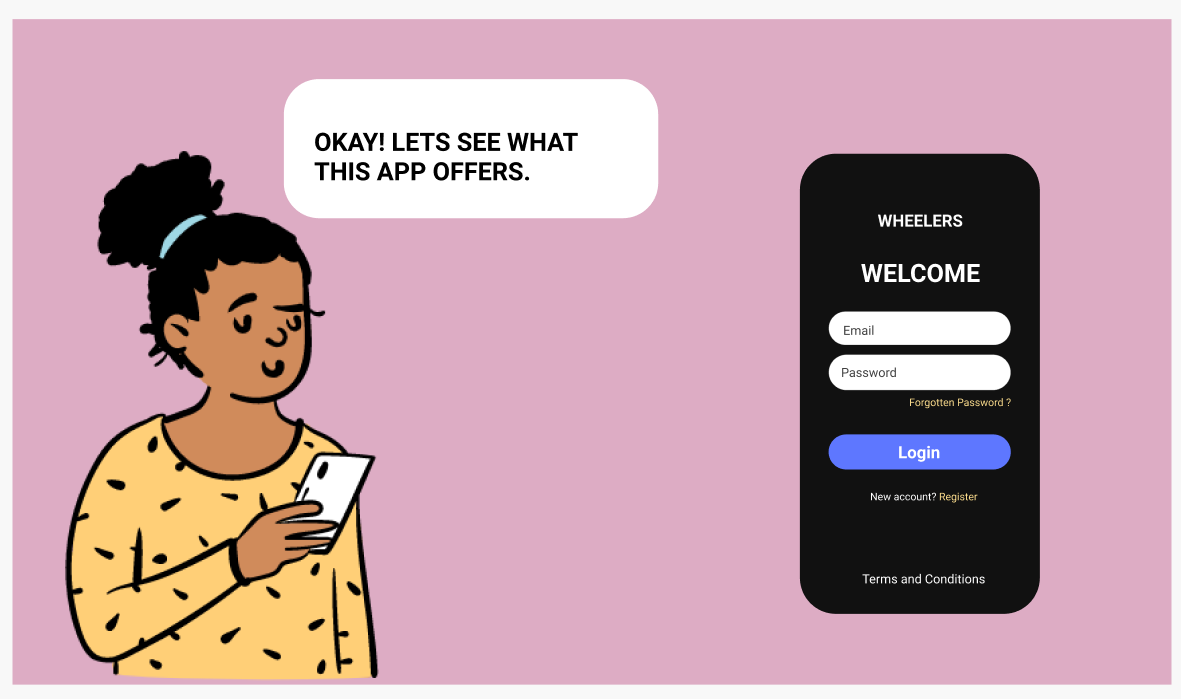
\includegraphics[width=1\textwidth]{images/3.png}
  \caption{3 Digital storyboard}
 \end{minipage}%
 \begin{minipage}[b]{0.55\textwidth}
  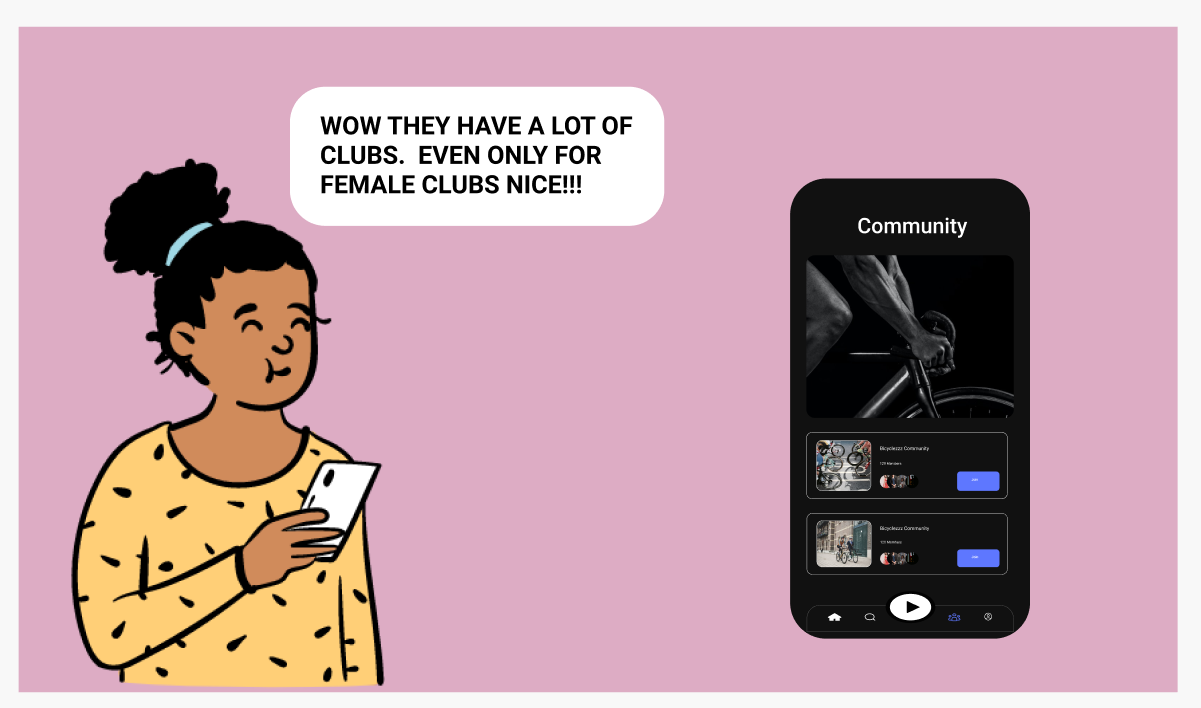
\includegraphics[width=1\textwidth]{images/4.png}
  \caption{4 Digital storyboard}
 \end{minipage}
\end{figure}


\begin{figure}
 \centering
 \begin{minipage}[b]{0.55\textwidth}
  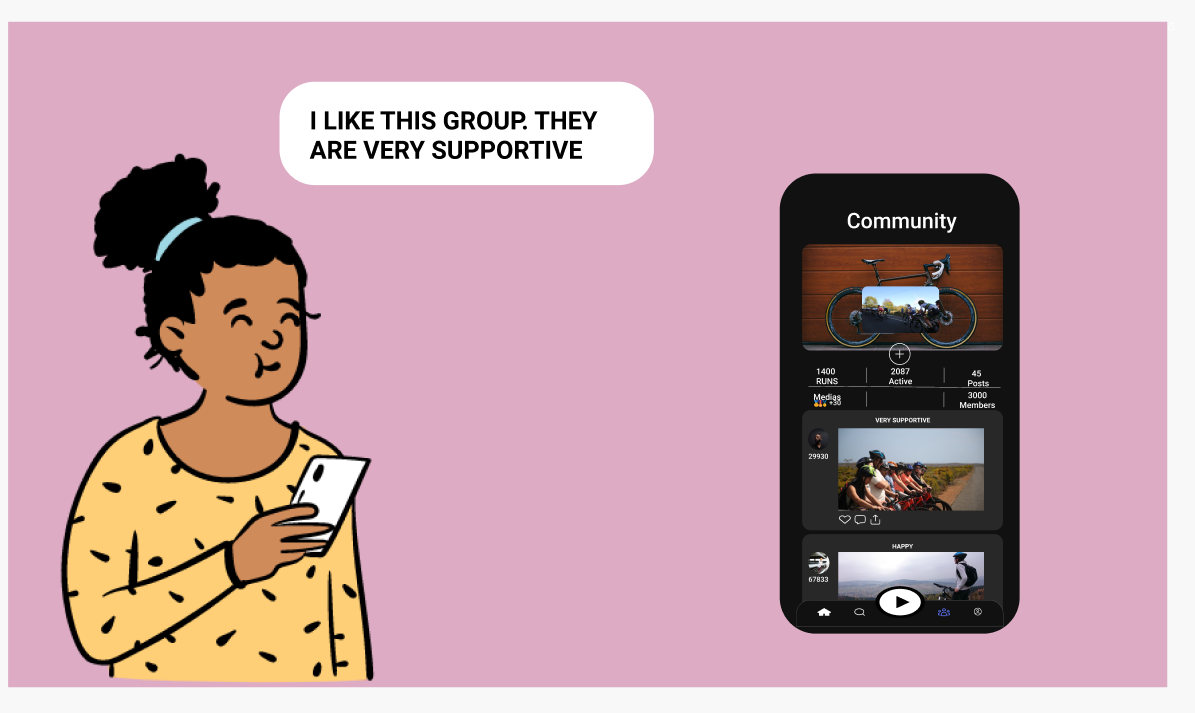
\includegraphics[width=1\textwidth]{images/5.png}
  \caption{5 Digital storyboard}
 \end{minipage}%
 \begin{minipage}[b]{0.55\textwidth}
  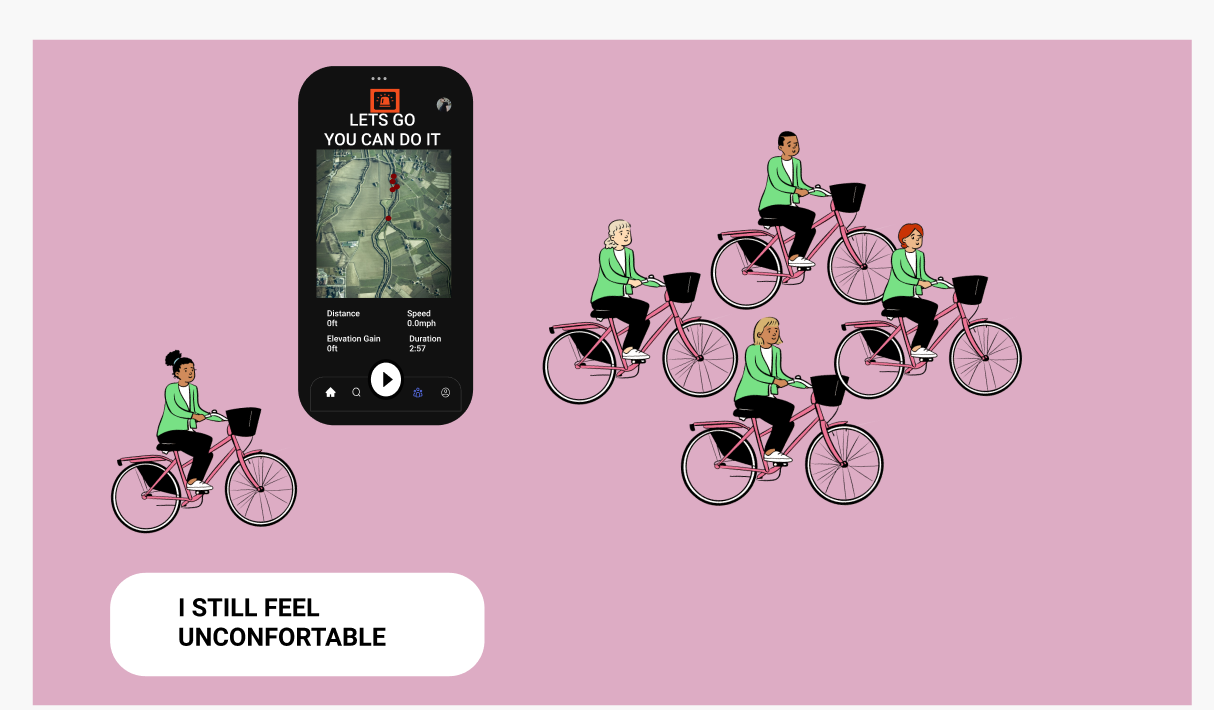
\includegraphics[width=1\textwidth]{images/6.png}
  \caption{6 Digital storyboard}
 \end{minipage}
\end{figure}


\begin{figure}
 \centering
 \begin{minipage}[b]{0.55\textwidth}
  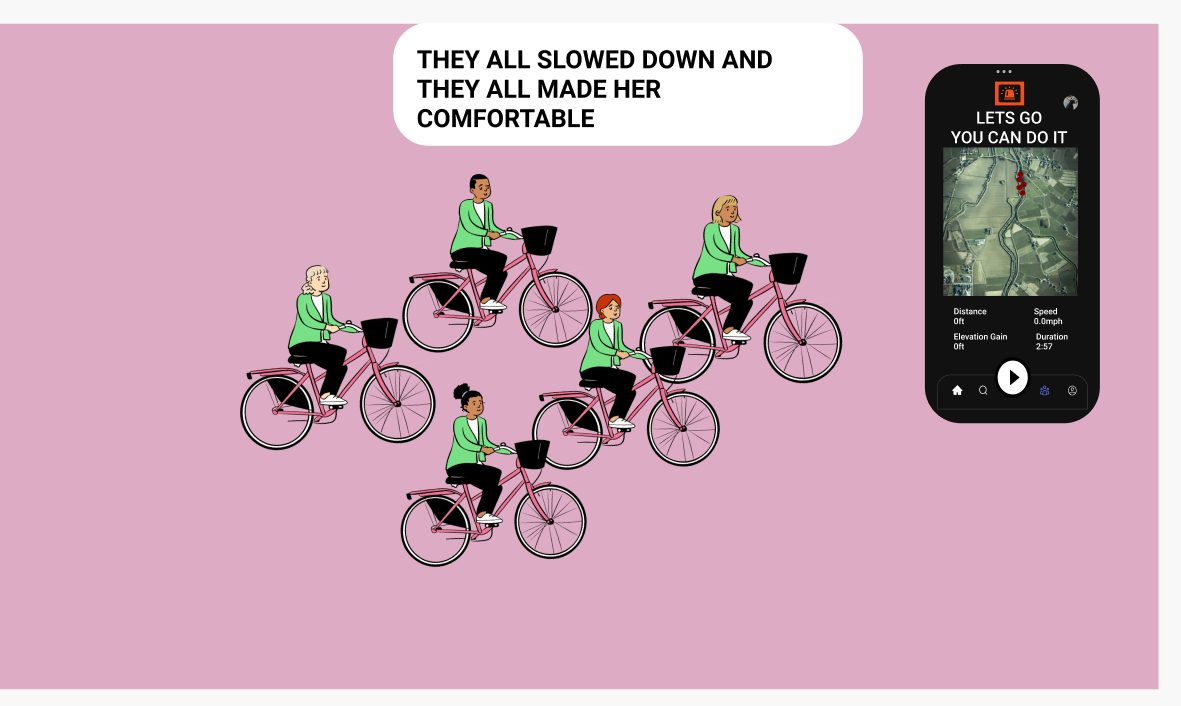
\includegraphics[width=1\textwidth]{images/7.png}
  \caption{7 Digital storyboard}
 \end{minipage}%
 \begin{minipage}[b]{0.55\textwidth}
  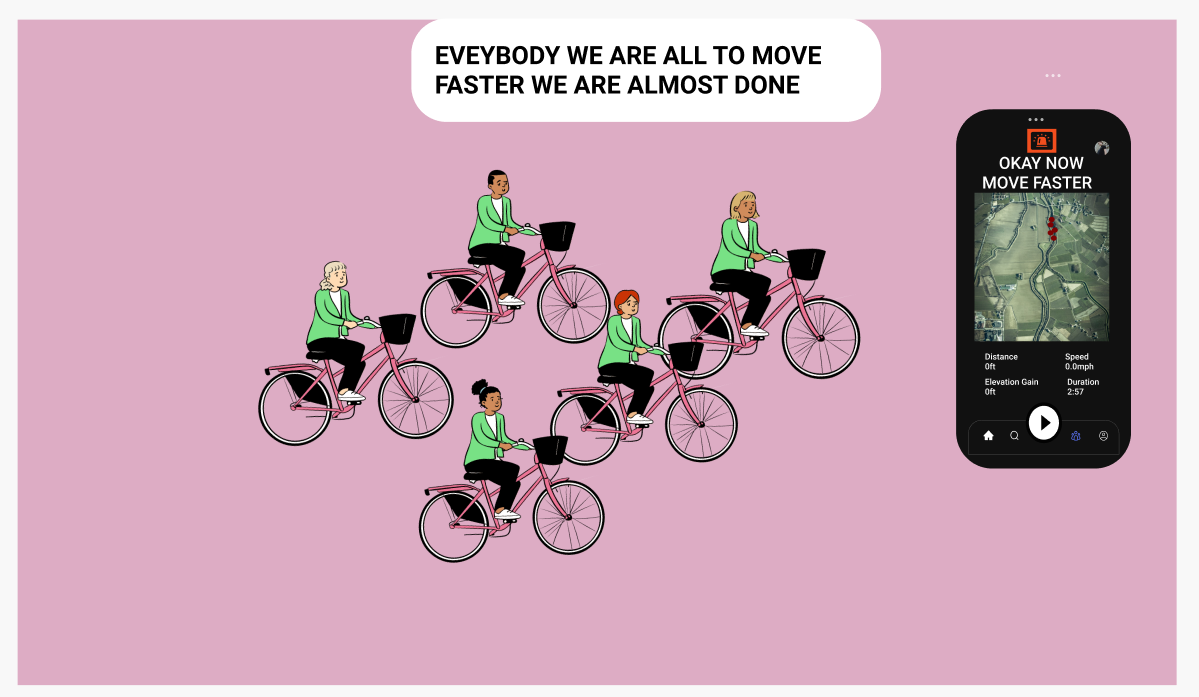
\includegraphics[width=1\textwidth]{images/8.png}
  \caption{8 Digital storyboard}
 \end{minipage}
\end{figure}

\begin{figure}
 \centering
 \begin{minipage}[b]{0.55\textwidth}
  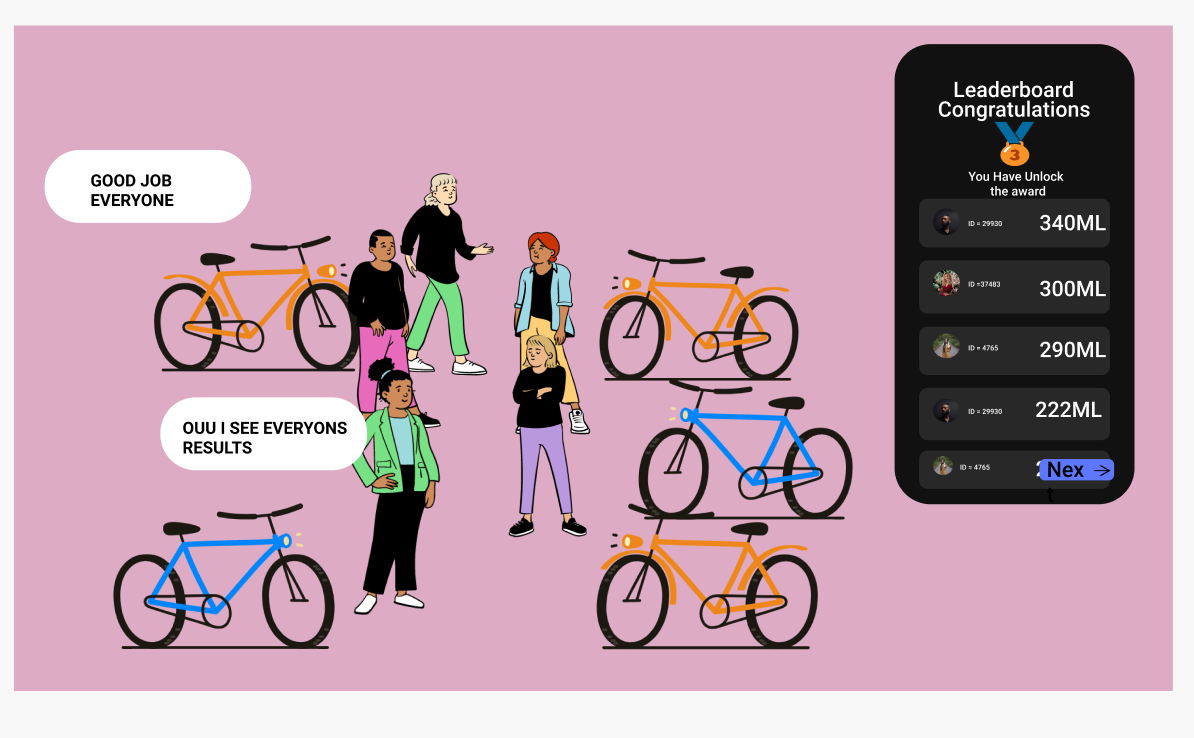
\includegraphics[width=1\textwidth]{images/9.png}
  \caption{9 Digital storyboard}
 \end{minipage}%
\end{figure}



\section{Guidance}
This chapter looks to provide insight into the technical implementation of the design outlined in \textbf{Chapter \ref{Design}}. We will look into the different frameworks and architectures implemented.

\section{Front-End implementation details}
A major part in development resources was the iOS application that was developed as part of the implementation.Thus part will discuss about the front-end implementation of the whole project.The front end is everything you see and can interact with. So, creating this visual part is called front-end development. The front-end is what a user sees and interacts with (user interface). The back-end is part of the application that is hidden from the user (what some would call, under the hood). This part is responsible for data processing, storing the data, and mathematical operations You could even say that designers creating user interfaces and planning experiences are also front-end developers, as they are working in collaboration on the same part of the project. The emphasis of this project lies within in the evaluation of the different stages of development rather than the implementation details and therefore some aspects of the design have been contorted to fit within the scope and limitations of the project.

\begin{figure}
    \centering
     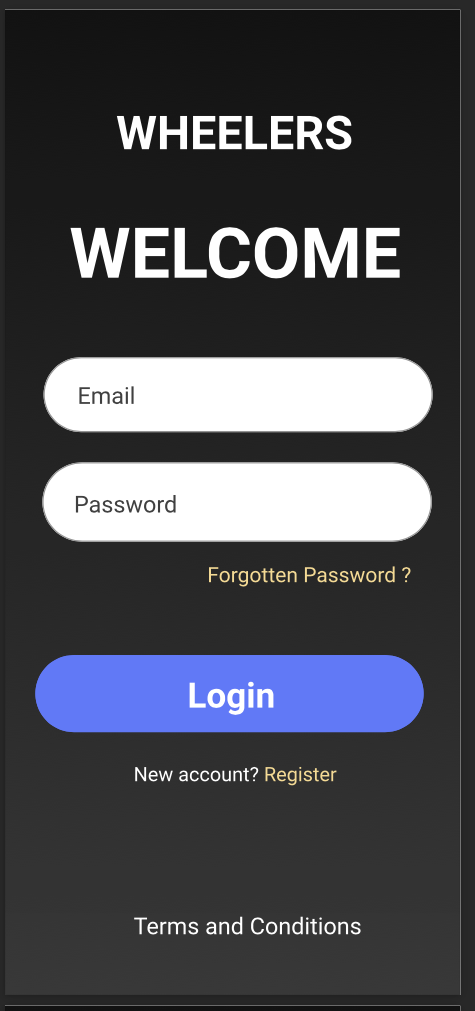
\includegraphics[width=.3\textwidth]{images/Screenshot 2022-02-15 at 1.49.53 pm.png}
     \caption{Prototype}
    \label{fig:my_label}
\end{figure}

\newpage
\subsection{React Native}
The programming language chosen was React Native, React Native is an open-source UI software framework created by Meta Platforms, Inc. It is used to develop applications for Android, Android TV, iOS, macOS, tvOS, Web, Windows and UWP by enabling developers to use the React framework along with native platform capabilities.React primitives render to native platform UI, meaning your app uses the same native platform APIs other apps do.The Seamless Cross-Platform React components wrap existing native code and interact with native APIs via React’s declarative UI paradigm and JavaScript. Js/React is an open-source frontend framework that is based on JavaScript, developed by Facebook, and best known for its virtual DOM feature. With React, we recommend Express. js/Express as a backend service. Previously, Swift was one of the first language used for this app. This language was suggested by many others. Even after being seven years old that has already gained a lot of traction in mobile app development. React Native was easier to navigate also was really familiar to JavaScript. React Native is a JavaScript framework created by the Facebook team to accelerate mobile development processes and build apps across platforms. In Swift vs React Native, the latter is supported by JavaScript which is the most popular language in the world, according to Statista. With almost 68 of developers’ support, JavaScript is way ahead of Swift in popularity and usage. React Native has benefits such as: Time efficiency,Rich library support, Gateway to nativeness, Performance and much more. Figure 5.2 shows every page must import react native and all the necessary tools needed. Creating the function and calling other pages to navigate to the pages. The navigation was a bit of a problem. With the help of a colleague it was able to work. There was a challenge with the stack navigator package. With previous knowledge from Human Computer Interaction (HCI), I was able to use the method to navigate from pages to pages. Although the design might be a bit odd the navigation still worked . 



\begin{figure}
    \centering
     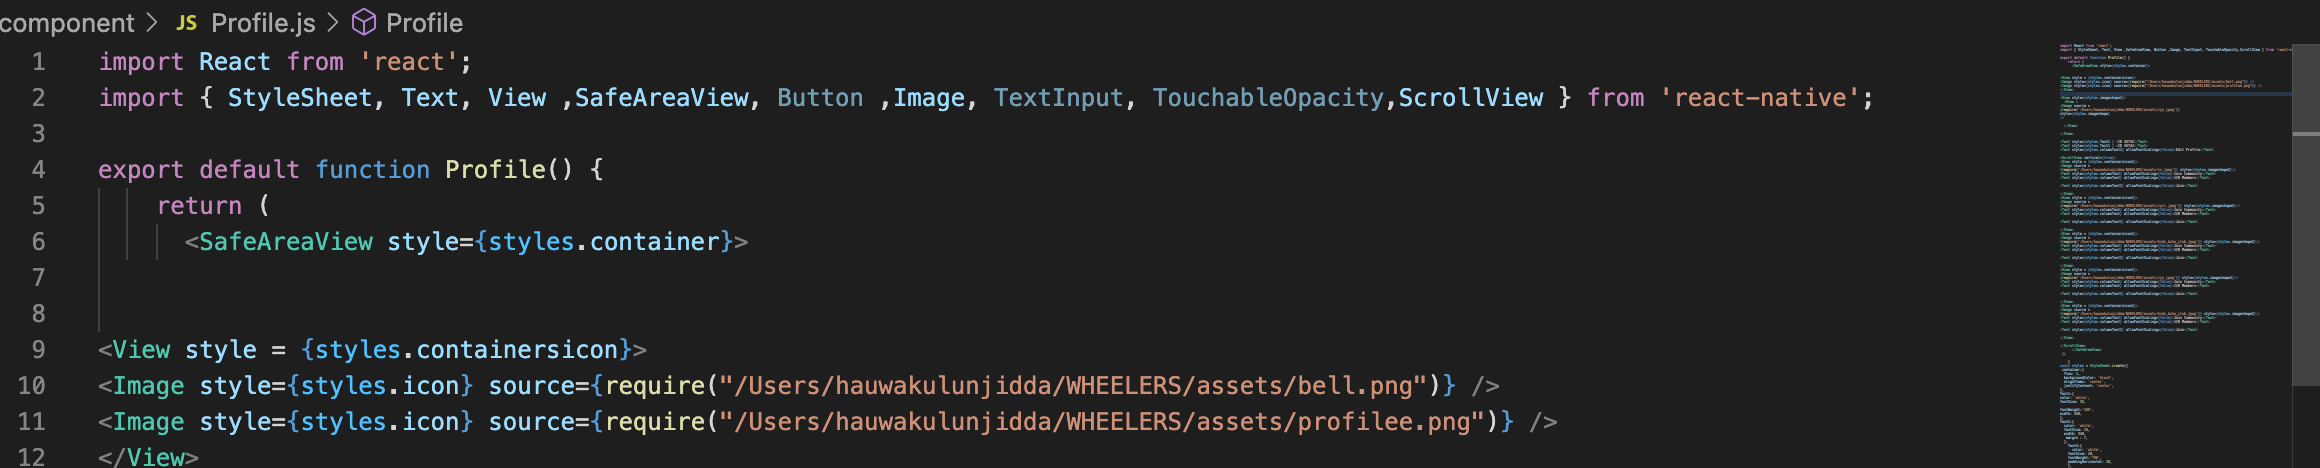
\includegraphics[width=1\textwidth]{images/q.png}
     \caption{Profile code }
    \label{fig:my_label}
\end{figure}

\begin{figure}
    \centering
        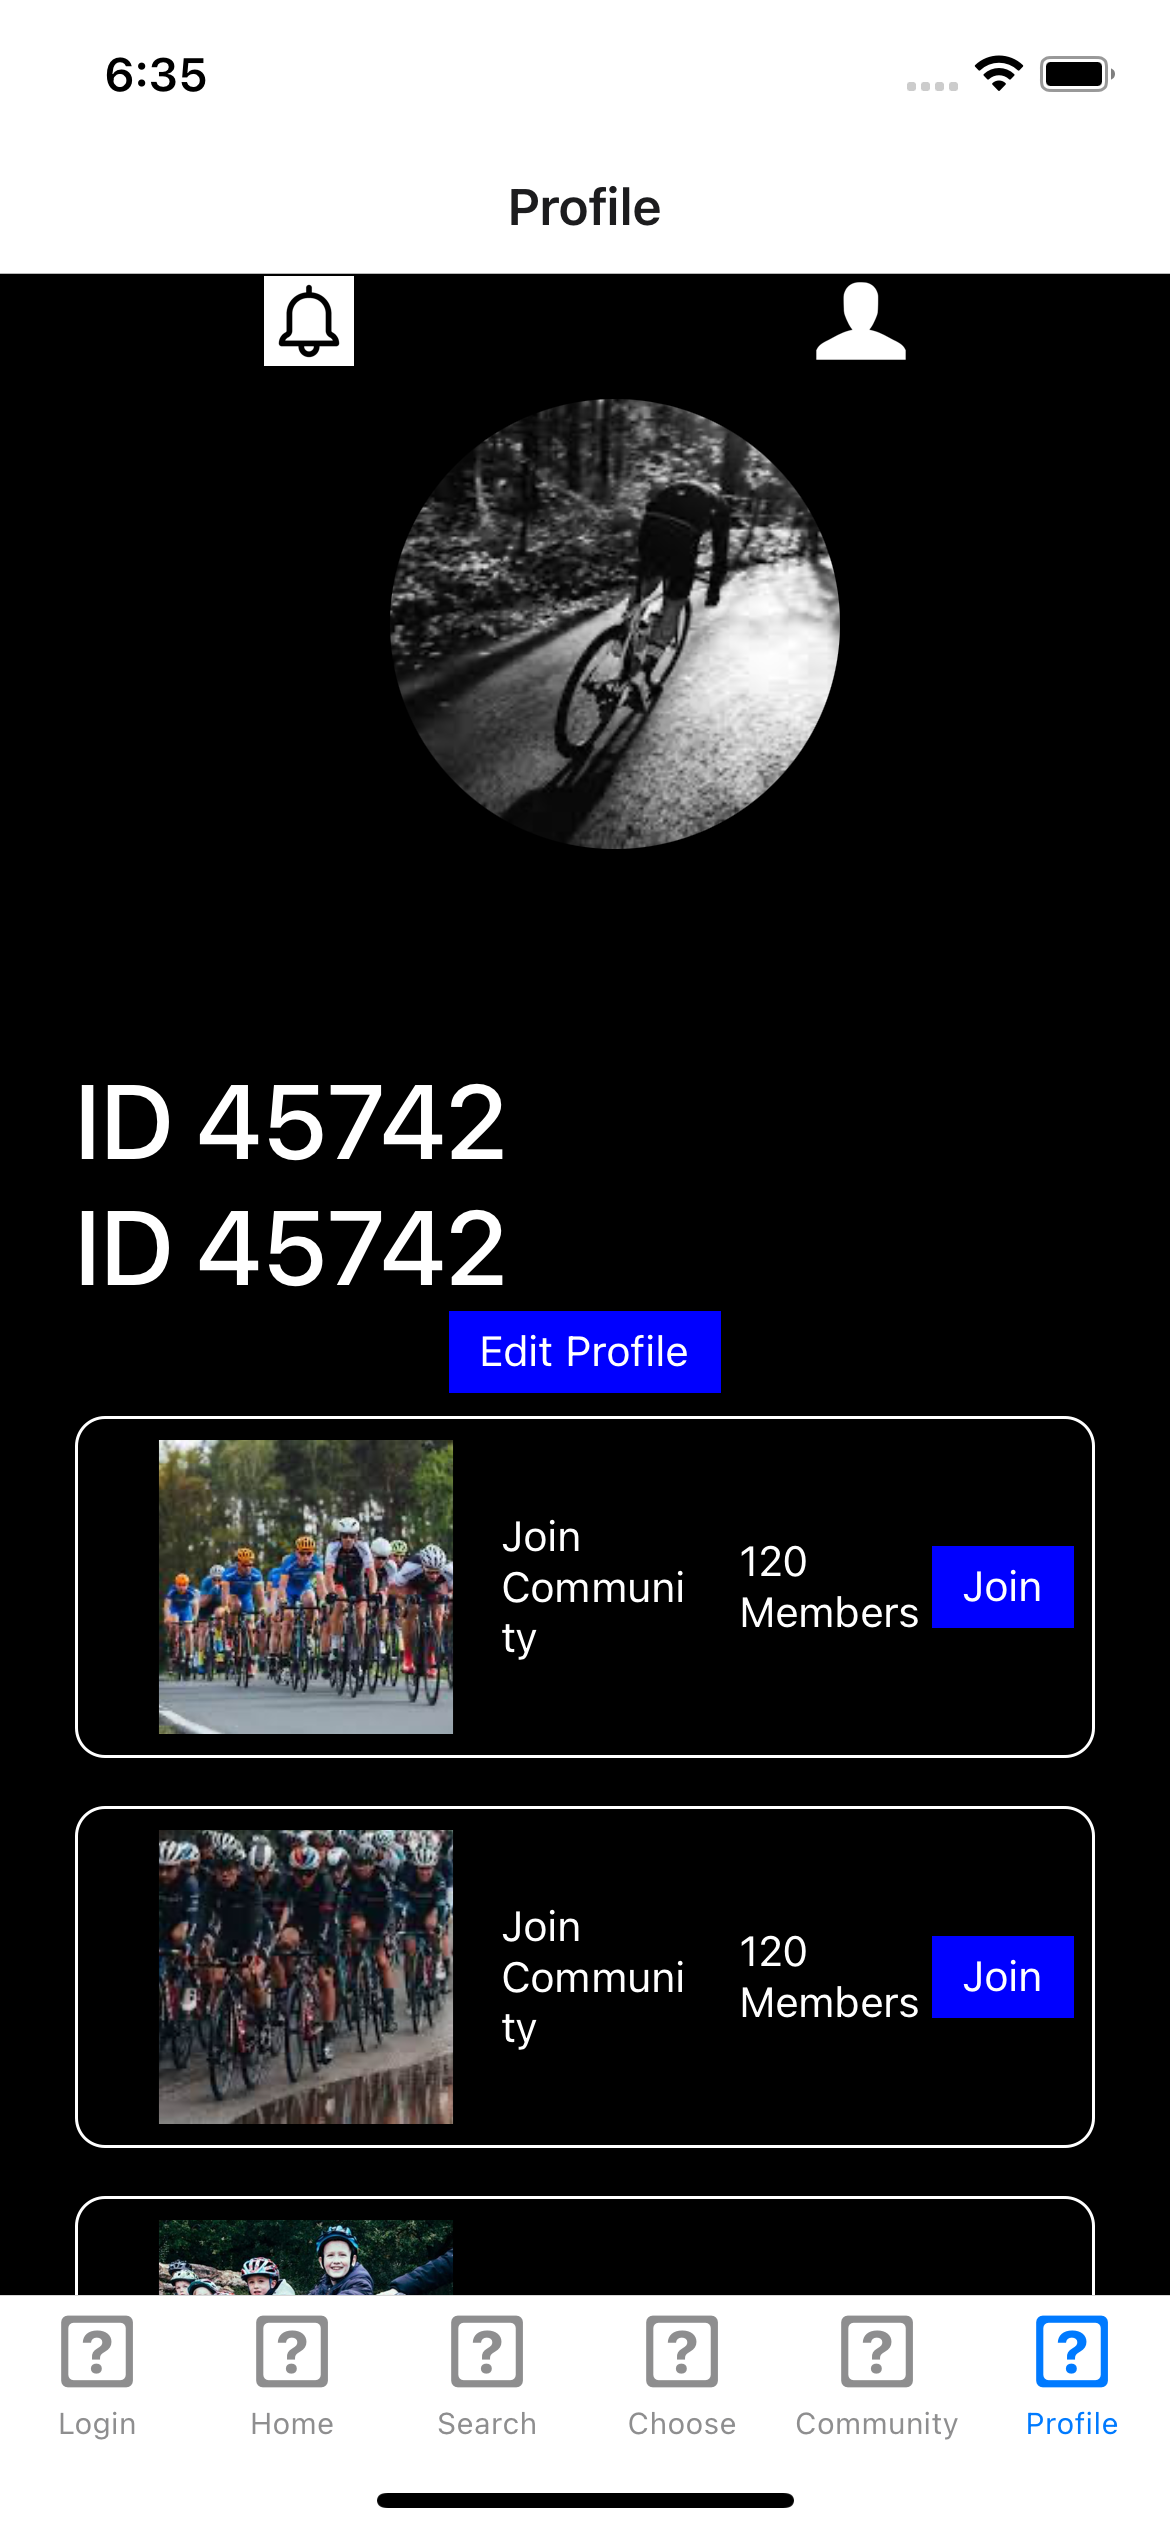
\includegraphics[scale=0.19]{images/999.png}
     \caption{Profile screen }
    \label{fig:my_label}
\end{figure}

\begin{figure}
    \centering
     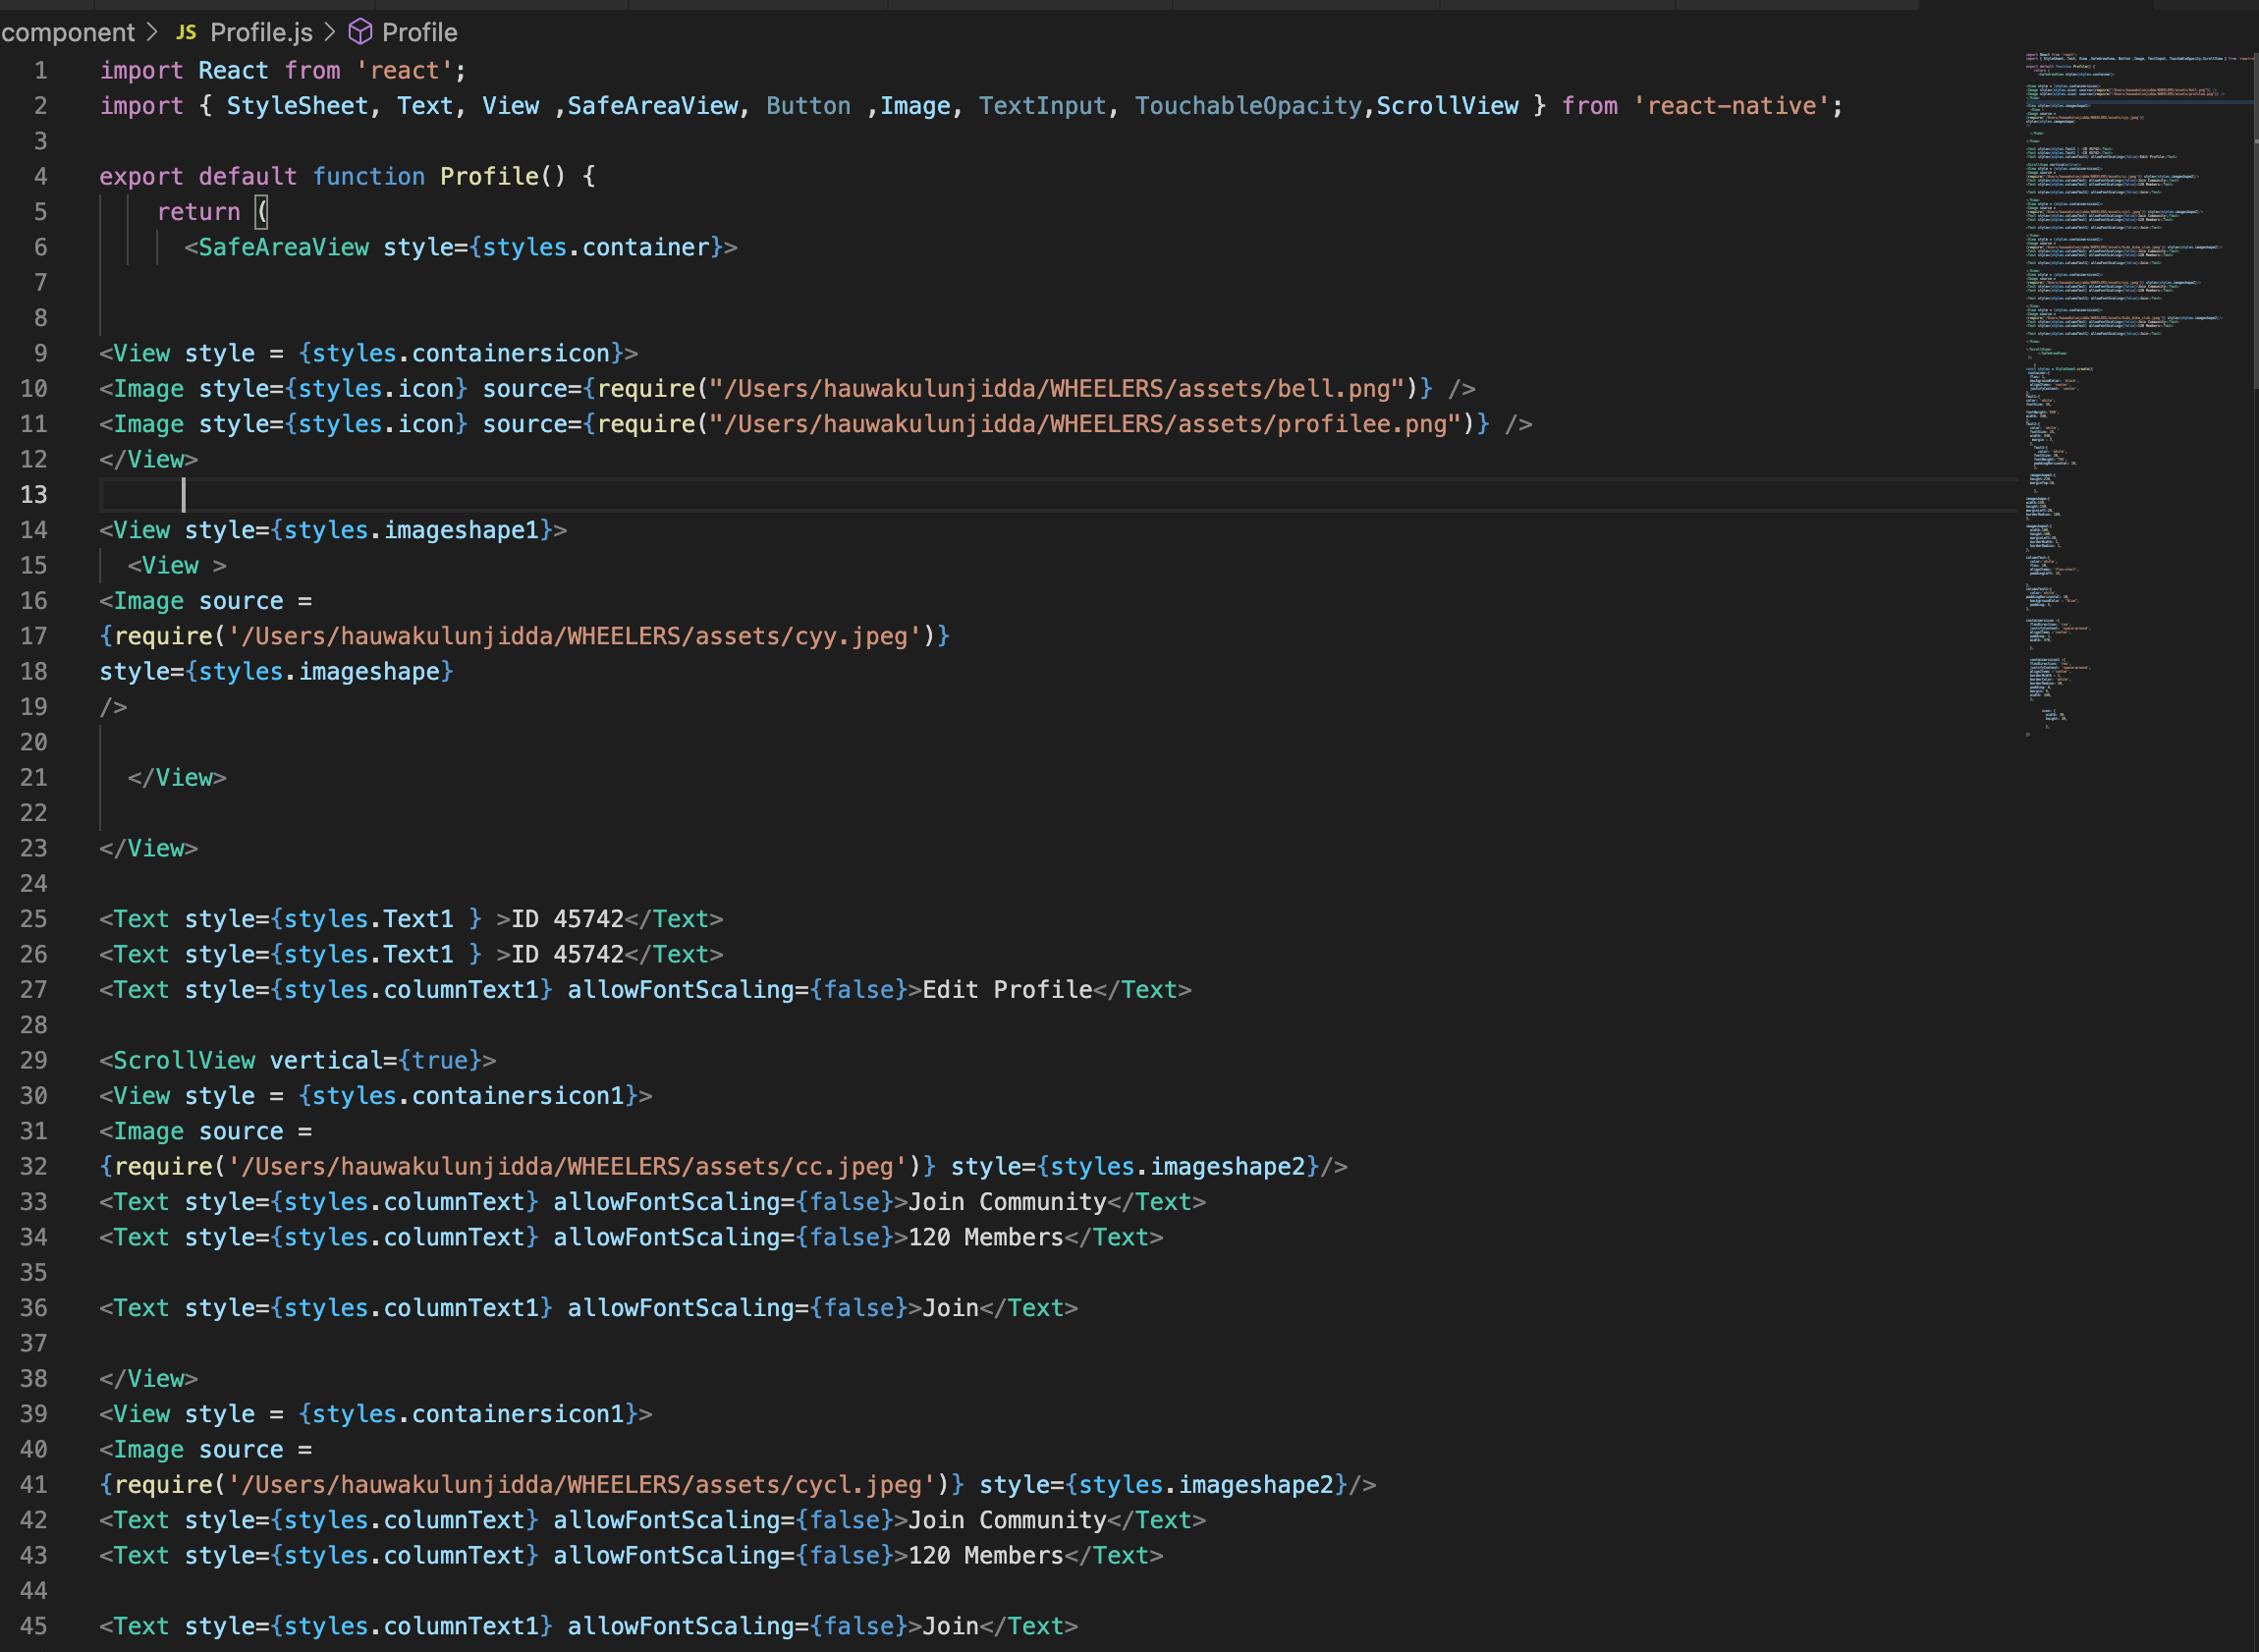
\includegraphics[width=1\textwidth]{images/98.png}
     \caption{React Native}
    \label{fig:my_label}
\end{figure}

\chapter{Evaluation} 
 

\section{Stages of Evaluations } 
The paper prototype was used to run some evaluations. As the projects moves on from paper prototype to figma prototype with different stages of evaluation. The evaluation was used to update and adjust the project. This section will discuss more about the evolution and the stages and types of testing taken.


\subsection{10 Usability Heuristics }
\label{HeuristicEvaluation}
 

Heuristic evaluation is a process where experts use rules of thumb to measure the usability of user interfaces in independent walkthroughs and report issues. Evaluators use established heuristics (e.g., Nielsen-Molich's) and reveal insights that can help design teams enhance product usability from early in development. The early deign process Jacob Nielsen's Laws was used, even after the paper prototype was not fully complete. The main designs were the already apps which are STRAVA, MapMyRide, RideWithGPS.

\textbf{Visibility of system status}: The Starva had no  visibilty of system status, for example the home page of starva shows  nothing. This does not explain why the screen is blank.





\textbf{Match between system and the real world}:The system should speak the users' language, with words, phrases and concepts familiar to the user, rather than system-oriented terms. The way you should design depends very much on your specific users. Terms, concepts, icons, and images that seem perfectly clear to you and your colleagues may be unfamiliar or confusing to your users.Just like the apps above STRAVA, MapMyRide, RideWithGPS all show and speaks to the user. For example the user will like to go out and ride his bike. Clicking the start button signifies to start padding to that the track can be recorded. To evaluate whether this would be effective a more advanced prototype and evaluation method would be required.  

\textbf{User control and freedom}: In this proposed concept user control and freedom is relatively limited as the number of actions the user can perform are limited. When it's easy for people to back out of a process or undo an action, it fosters a sense of freedom and confidence. Exits allow users to remain in control of the system and avoid getting stuck and feeling frustrated. The user can pause his/her track and can go back to cancel it giving them the freedom to do so.

\textbf{Consistency and standards}: Users should not have to wonder whether different words, situations, or actions mean the same thing. Follow platform and industry conventions. The RideWithGPS had a clear flow towards everything there was no mixes of numbers. 
 

\textbf{Error prevention}: Good error messages are important, but the best designs carefully prevent problems from occurring in the first place. The prototype needs very little error prevention as there is little opportunity for the user to engage in user input. The prototype does showcase the ability to end the workout, which allows error prevention if it was started accidentally. 

\textbf{Recognition rather than recall}: Minimize the user's memory load by making elements, actions, and options visible. The app seems to perform well for this category. This can be done by simply clicking the play button. 

\textbf{Flexibility and efficiency of use}: Shortcuts — hidden from novice users — may speed up the interaction for the expert user such that the design can cater to both inexperienced and experienced users. Allow users to tailor frequent actions.Being that most of the apps using it requires an extra upgrade to get this future. Easy to navigate making it a bit hard for novice users. 

\textbf{Aesthetic and minimalist design}: The designs appears to be simple and straightforward.  
\begin{figure}[h!]
    \centering
    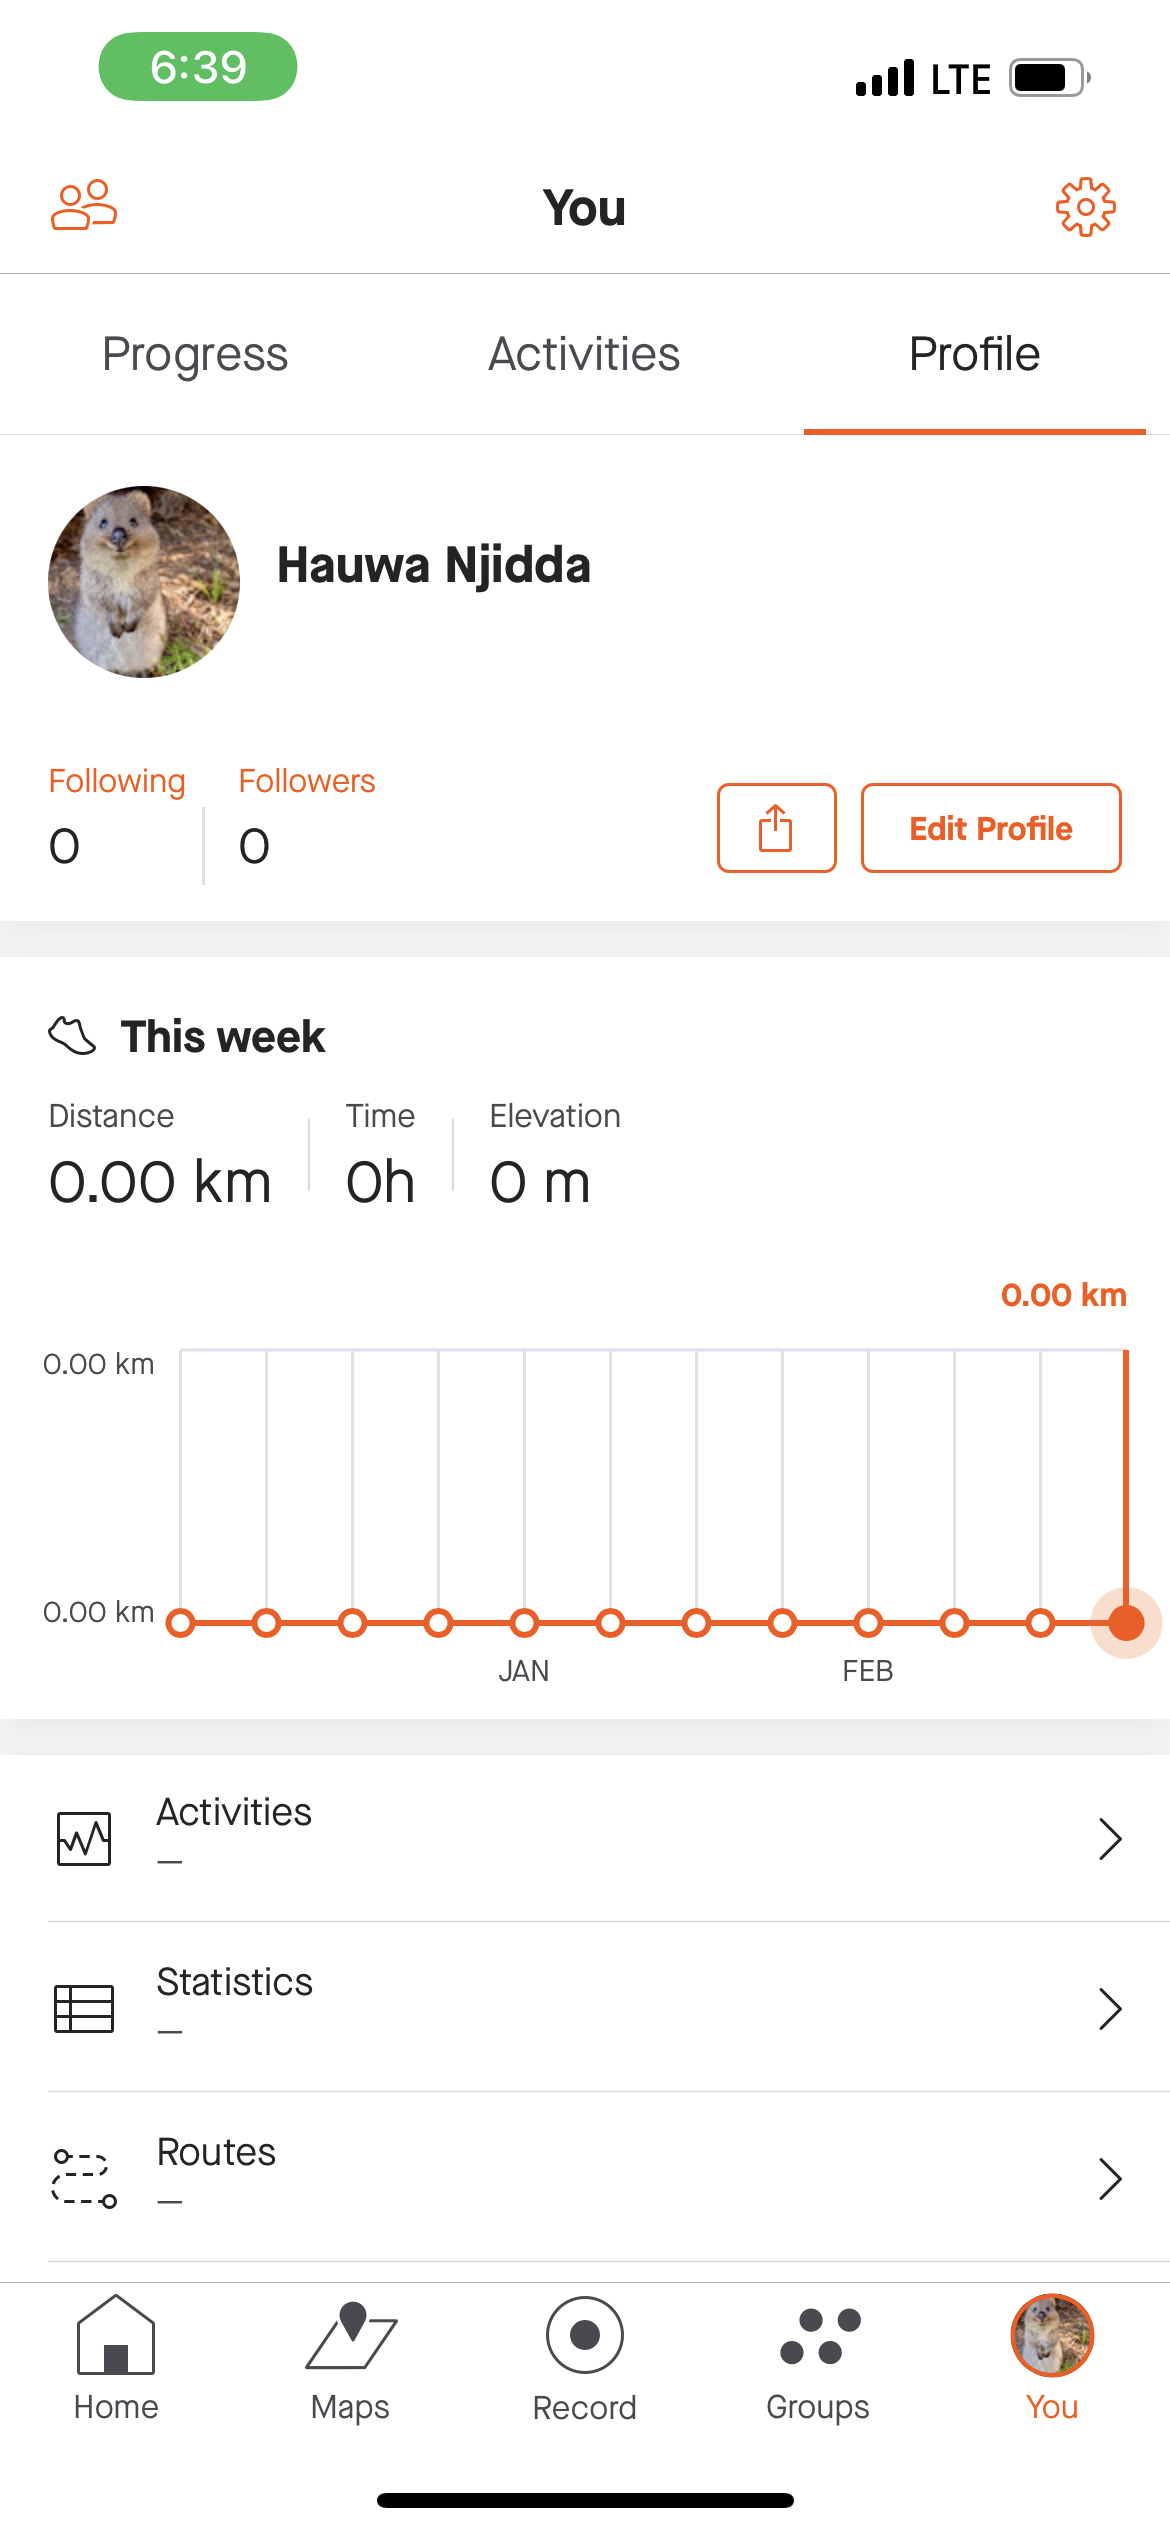
\includegraphics[scale=0.09]{images/STAR.PNG}
    \caption{Usability survey page one}
    \label{fig:surveypage1}
\end{figure}
\begin{figure}
 \centering
 \begin{minipage}[b]{0.3\textwidth}
  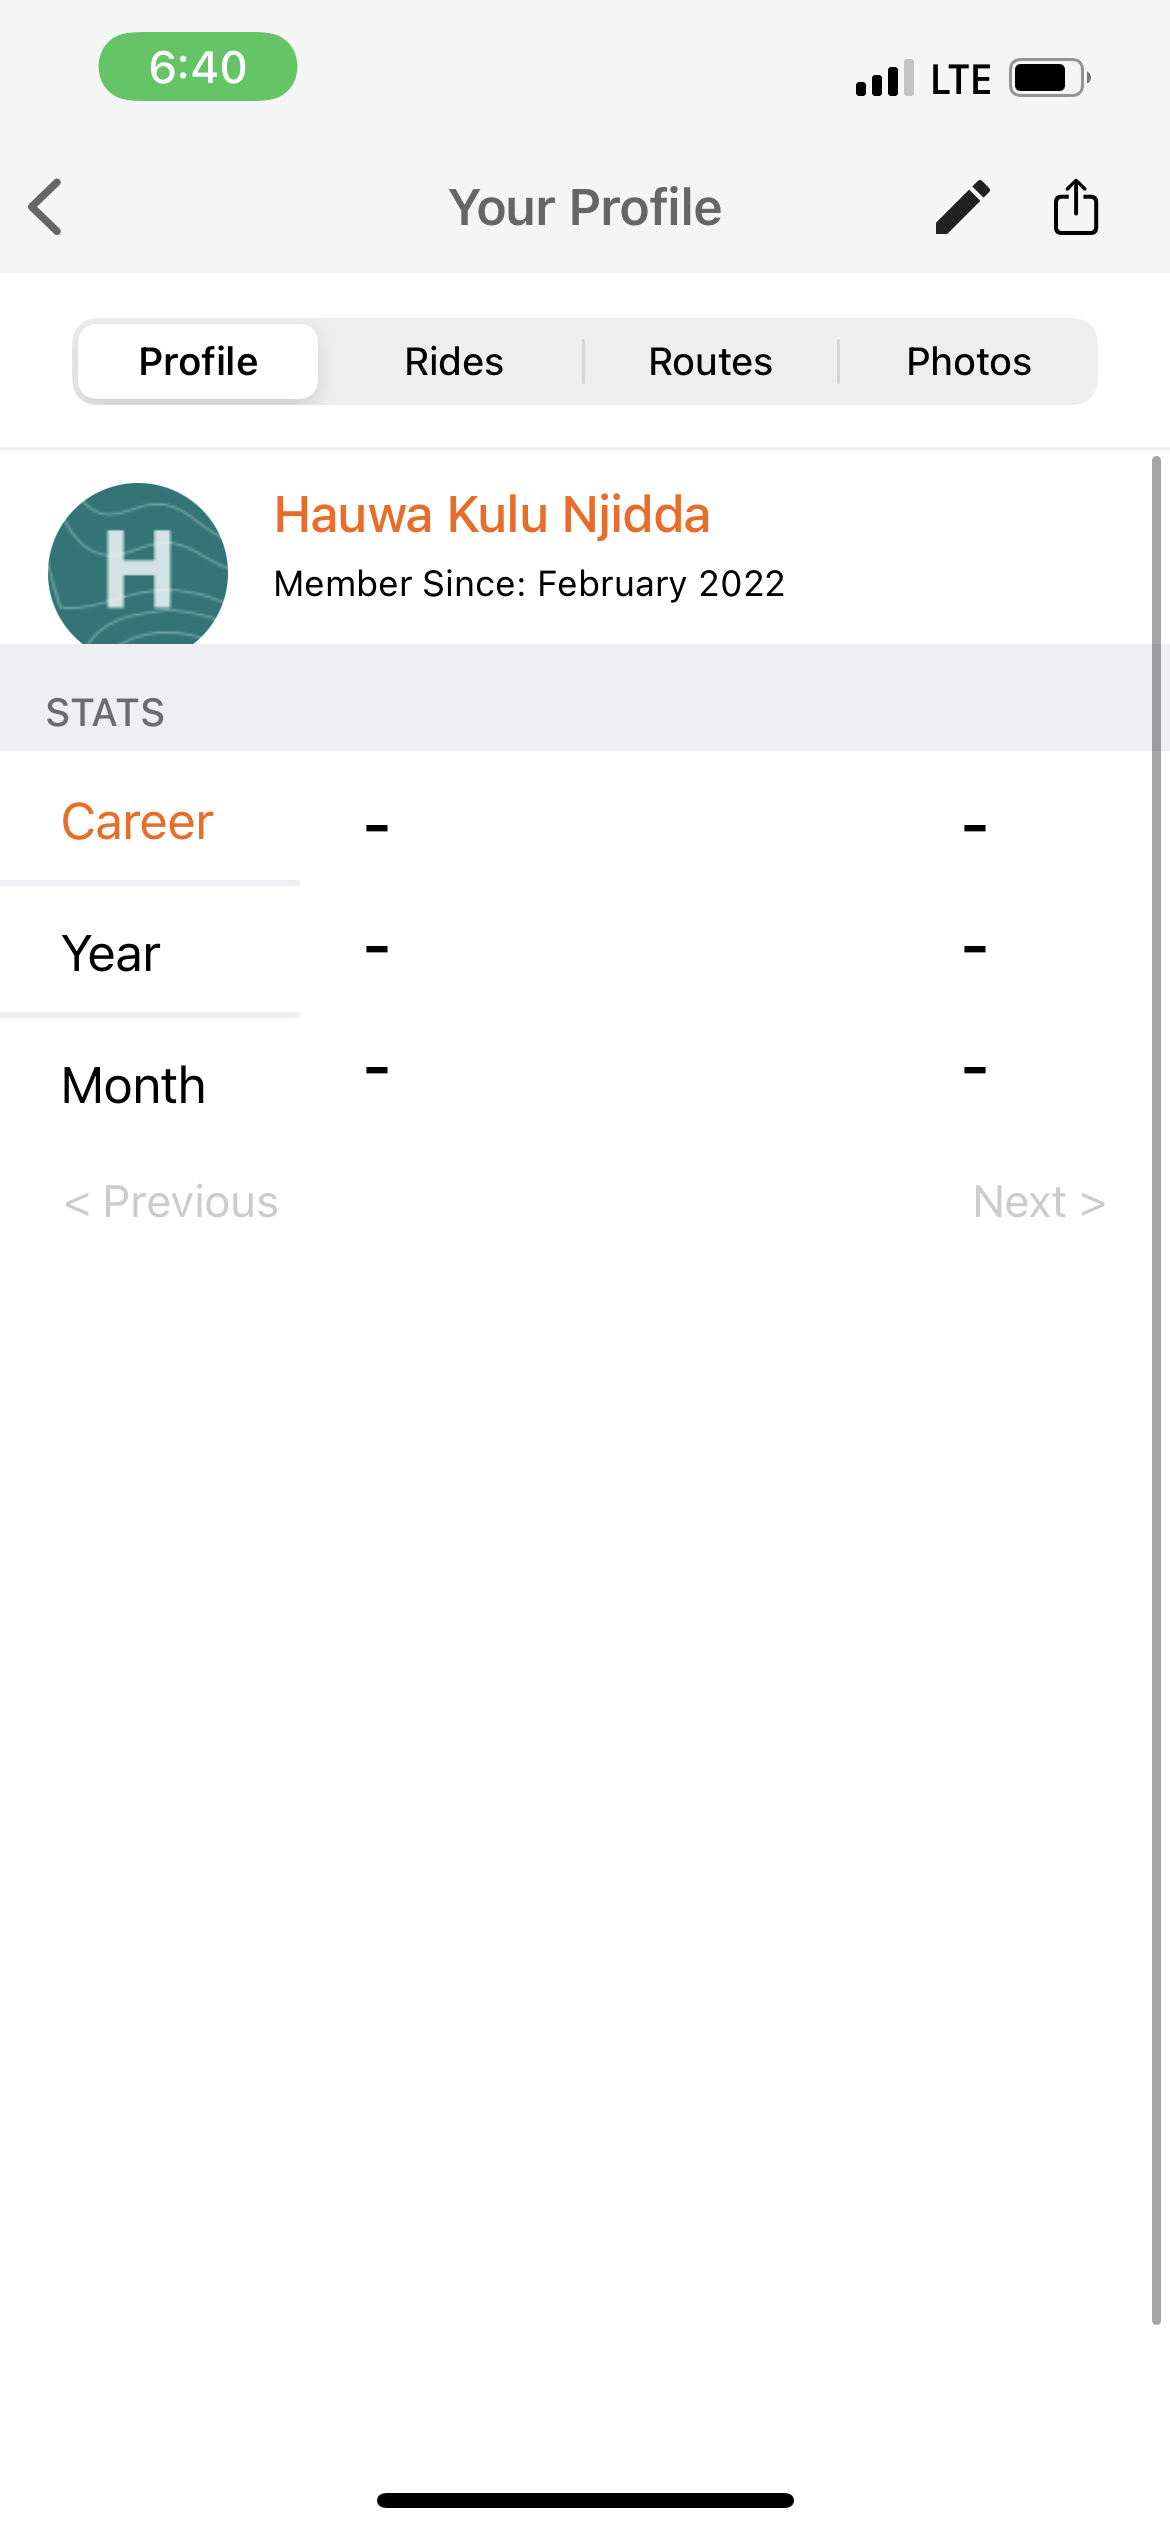
\includegraphics[width=1\textwidth]{images/NAM.PNG}
  \caption{Ride with GPS}
 \end{minipage}%
 \begin{minipage}[b]{0.3\textwidth}
  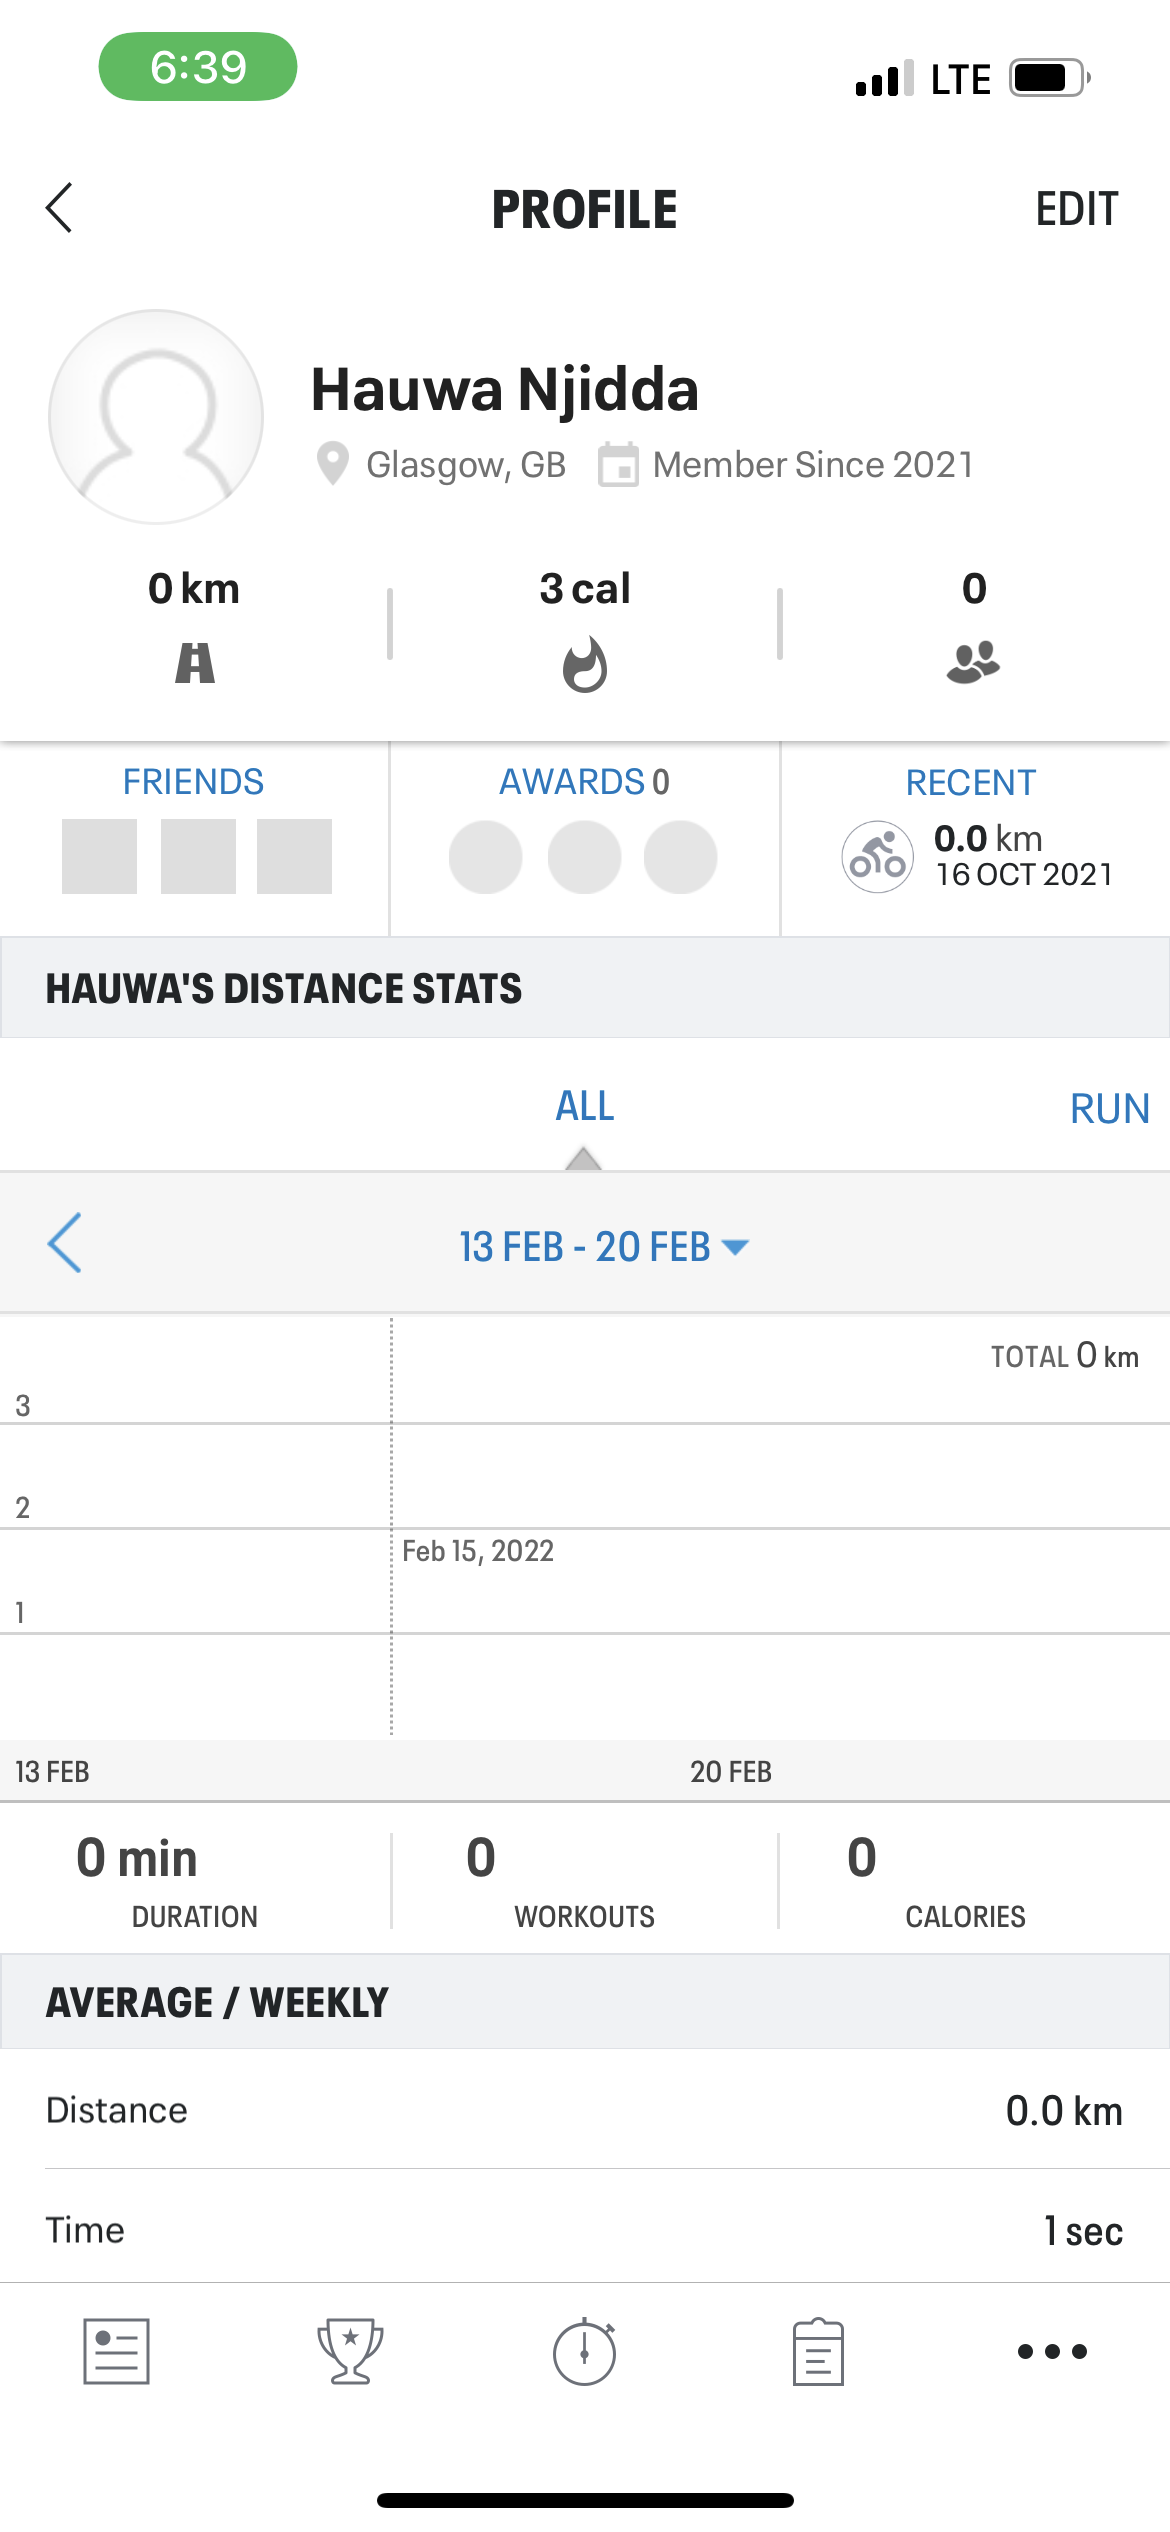
\includegraphics[width=1\textwidth]{images/MYPA.PNG}
  \caption{MapMyRide}
 \end{minipage}
 \begin{minipage}[b]{0.3\textwidth}
  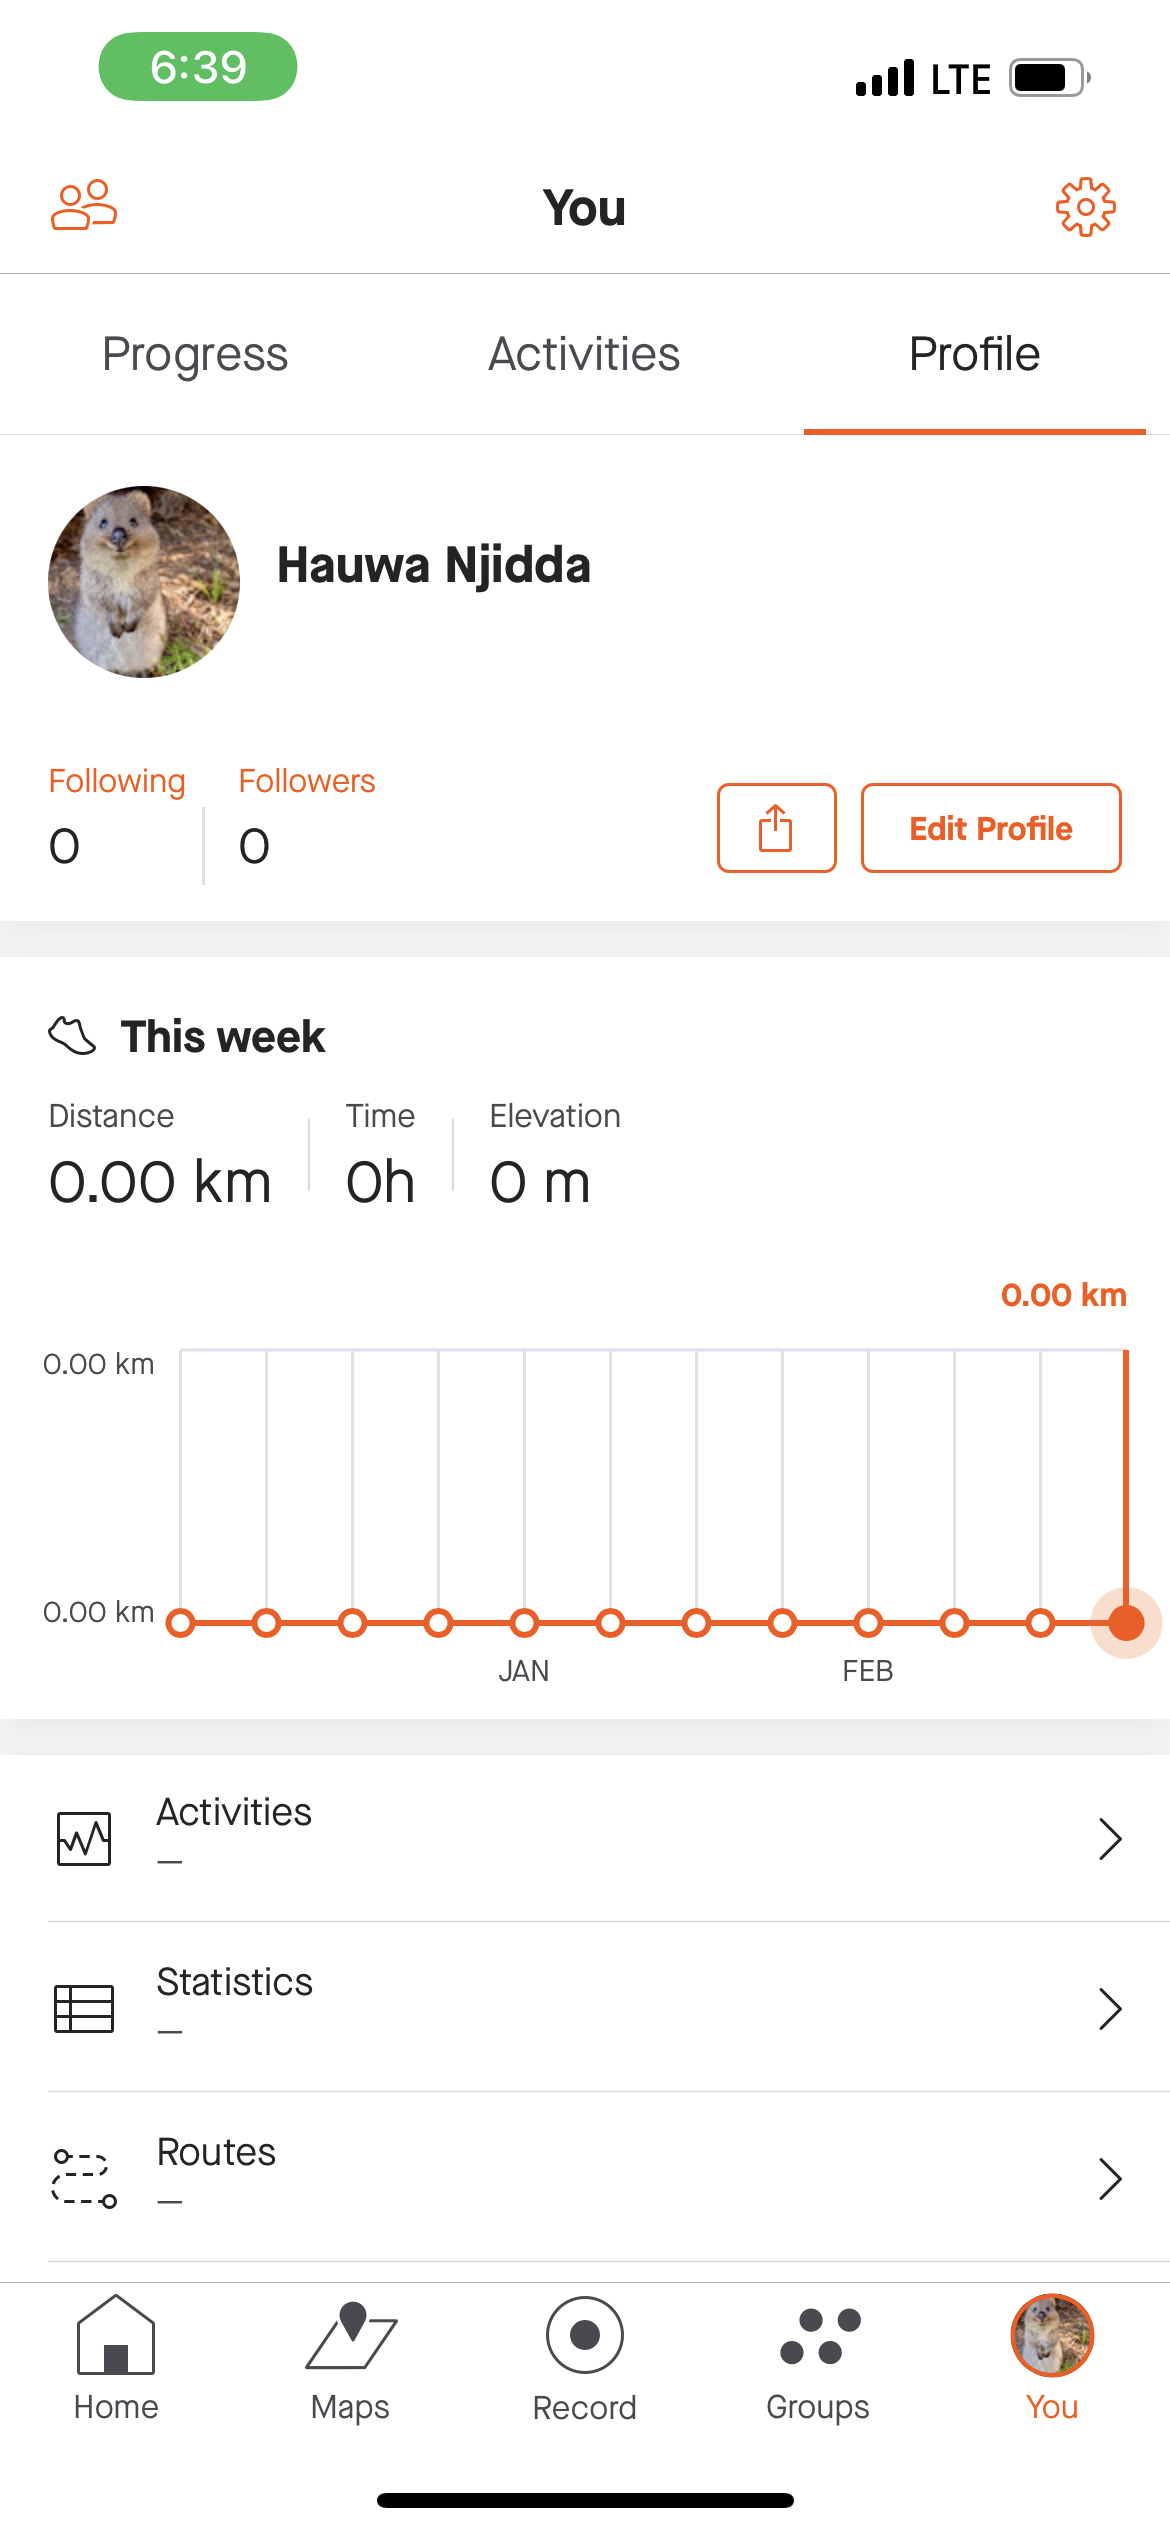
\includegraphics[width=1\textwidth]{images/STAR.PNG}
  \caption{Strava}
 \end{minipage}
 
\end{figure}


\subsection{Think-Aloud Evaluation} \label{ThinkAloud}
During iteration 2, a Think-Aloud evaluation was performed on the redesigned wireframes to gather feedback. This part will summarize the findings from the evaluation. The evaluation was run by three participants and they where shown the prototype of the WHEELERS app. as seen in \textbf{Figure \ref{fig:homepageprototype}}. 

The participants found the log in / create an account view easy to navigate and managed. The login page was easy to navigate the button was more visible than the register button however the participant recognised registered button just because of its colour being pronounced after clicking on the register button. The participants were instructed to act as if they had typed in an invalid email or password for which generic error feedback was displayed, prompting the participants to either fix their email or create a stronger password. It was clear as to what to type to complete the register page. Now going to the home screen which shows different ways and places and communities to join around your area. The users noted no issues with this interaction and iterated that the behaviour was expected and imitated that of most modern applications.


The participants then examined the home screen, now going to the home screen which shows different ways and places and communities to join around your area. The three participants noticed the types of places to bike near them and with how many it was to join a community right from the home page. All the participant all noticed the play button which was big enough and with base on the app they all knew the function and what it signifies.

The participants were then instructed to navigate to the search tab, which was shows the nearest and easiest bike tracking map . One participant suggested to explain the main purpose of having the search page rather than not showing anything. This means one of the participant did not understand the purpose of the search page. The users were instructed to try to track the location which landed no issue considering it was a prototype. 

The participants was later instructed attempt to click the play button. However, it automatically shows two options of the solo or group ride. One of the participant attempted the group ride, with then took her to the community group.As for the rest of the participants they considered the solo ride base on there observation a map was shown and started tracking there steps. This was easy to pause as it was visible and it was known in the real world. The next was to navigate to the community page. The participants exhibited no issue choosing  or picking the community they want. They were then navigated to go for a group ride with the group. This later shows the scores and was given a medal for participating and made it entertaining for the users to keep using the app. The engagement and interacting with others make the participants to keep using the app.

Overall, the participants found it fun and quite easy to navigate to other pages. 

\begin{figure}
    \centering
     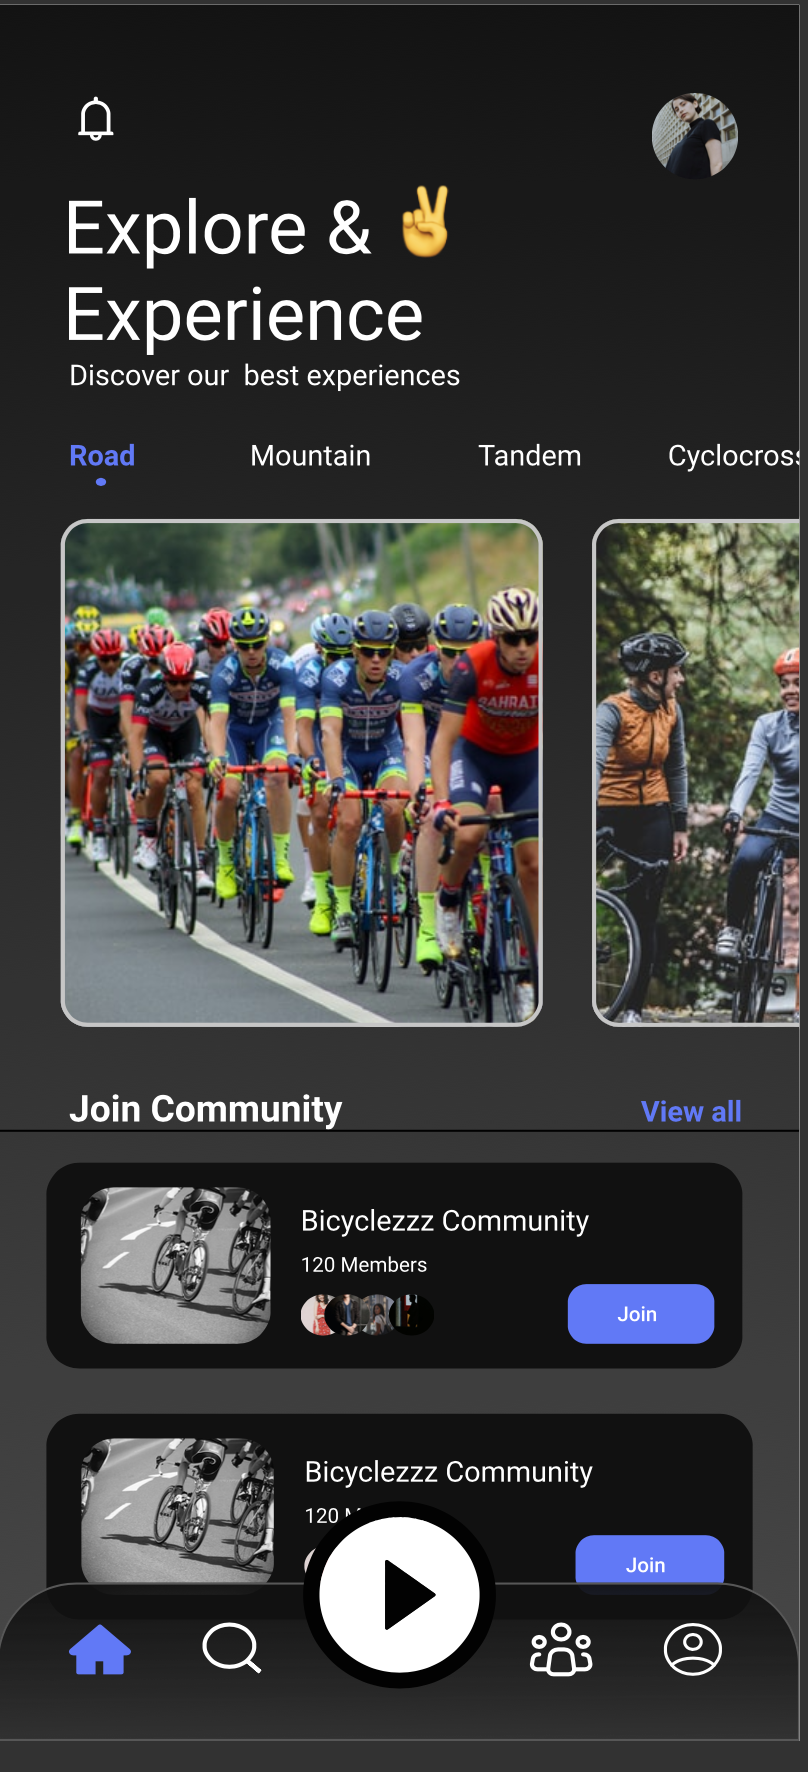
\includegraphics[width=0.4\textwidth]{images/Profile.png}
     \caption{Home page Prototype}
    \label{fig:homepageprototype}
\end{figure}

\section{Usability Testing}
With the evolution, it was important that the evaluation methods also evolved to cater for a more complete product. It was therefore important to perform some form of testing with users; for this project usability testing was identified as a suitable approach. The usability evaluation was run across a total of 3 weeks, comprising of 8 participants who where all students, Reaching out to cyclist was a bit difficult. The number of participants had an effect on some of the technical features of the app. The user testing itself was split into two weeks of actual use with additional time being allocated to evaluations such as surveys and interviews, as well time taken to implement new features identified from these evaluations. 



\subsection{Week 1}\label{UsabilityTestingWeekOne}
The first week of actual testing began with a few pre-test considerations; these included a think-aloud evaluation to ensure the app was functioning as expected which serves as a windows to the soul, ensuring the participation communication channels were set up, and finally briefing the users of expectations of the study and their rights as participants. 

As discussed previously, at the end of week 1 a survey was run to gather feedback and continue the iterative design process. The survey was flexible which was written down.  The survey revealed which features the users felt were lacking and were implemented before the second week of user testing. The think-aloud evaluation was also done by some of my close friends, to get more Information and gather them all in one. \textbf{Figure \ref{fig:Gettingideas}} shows the information form people.  
\begin{figure}
    \centering
     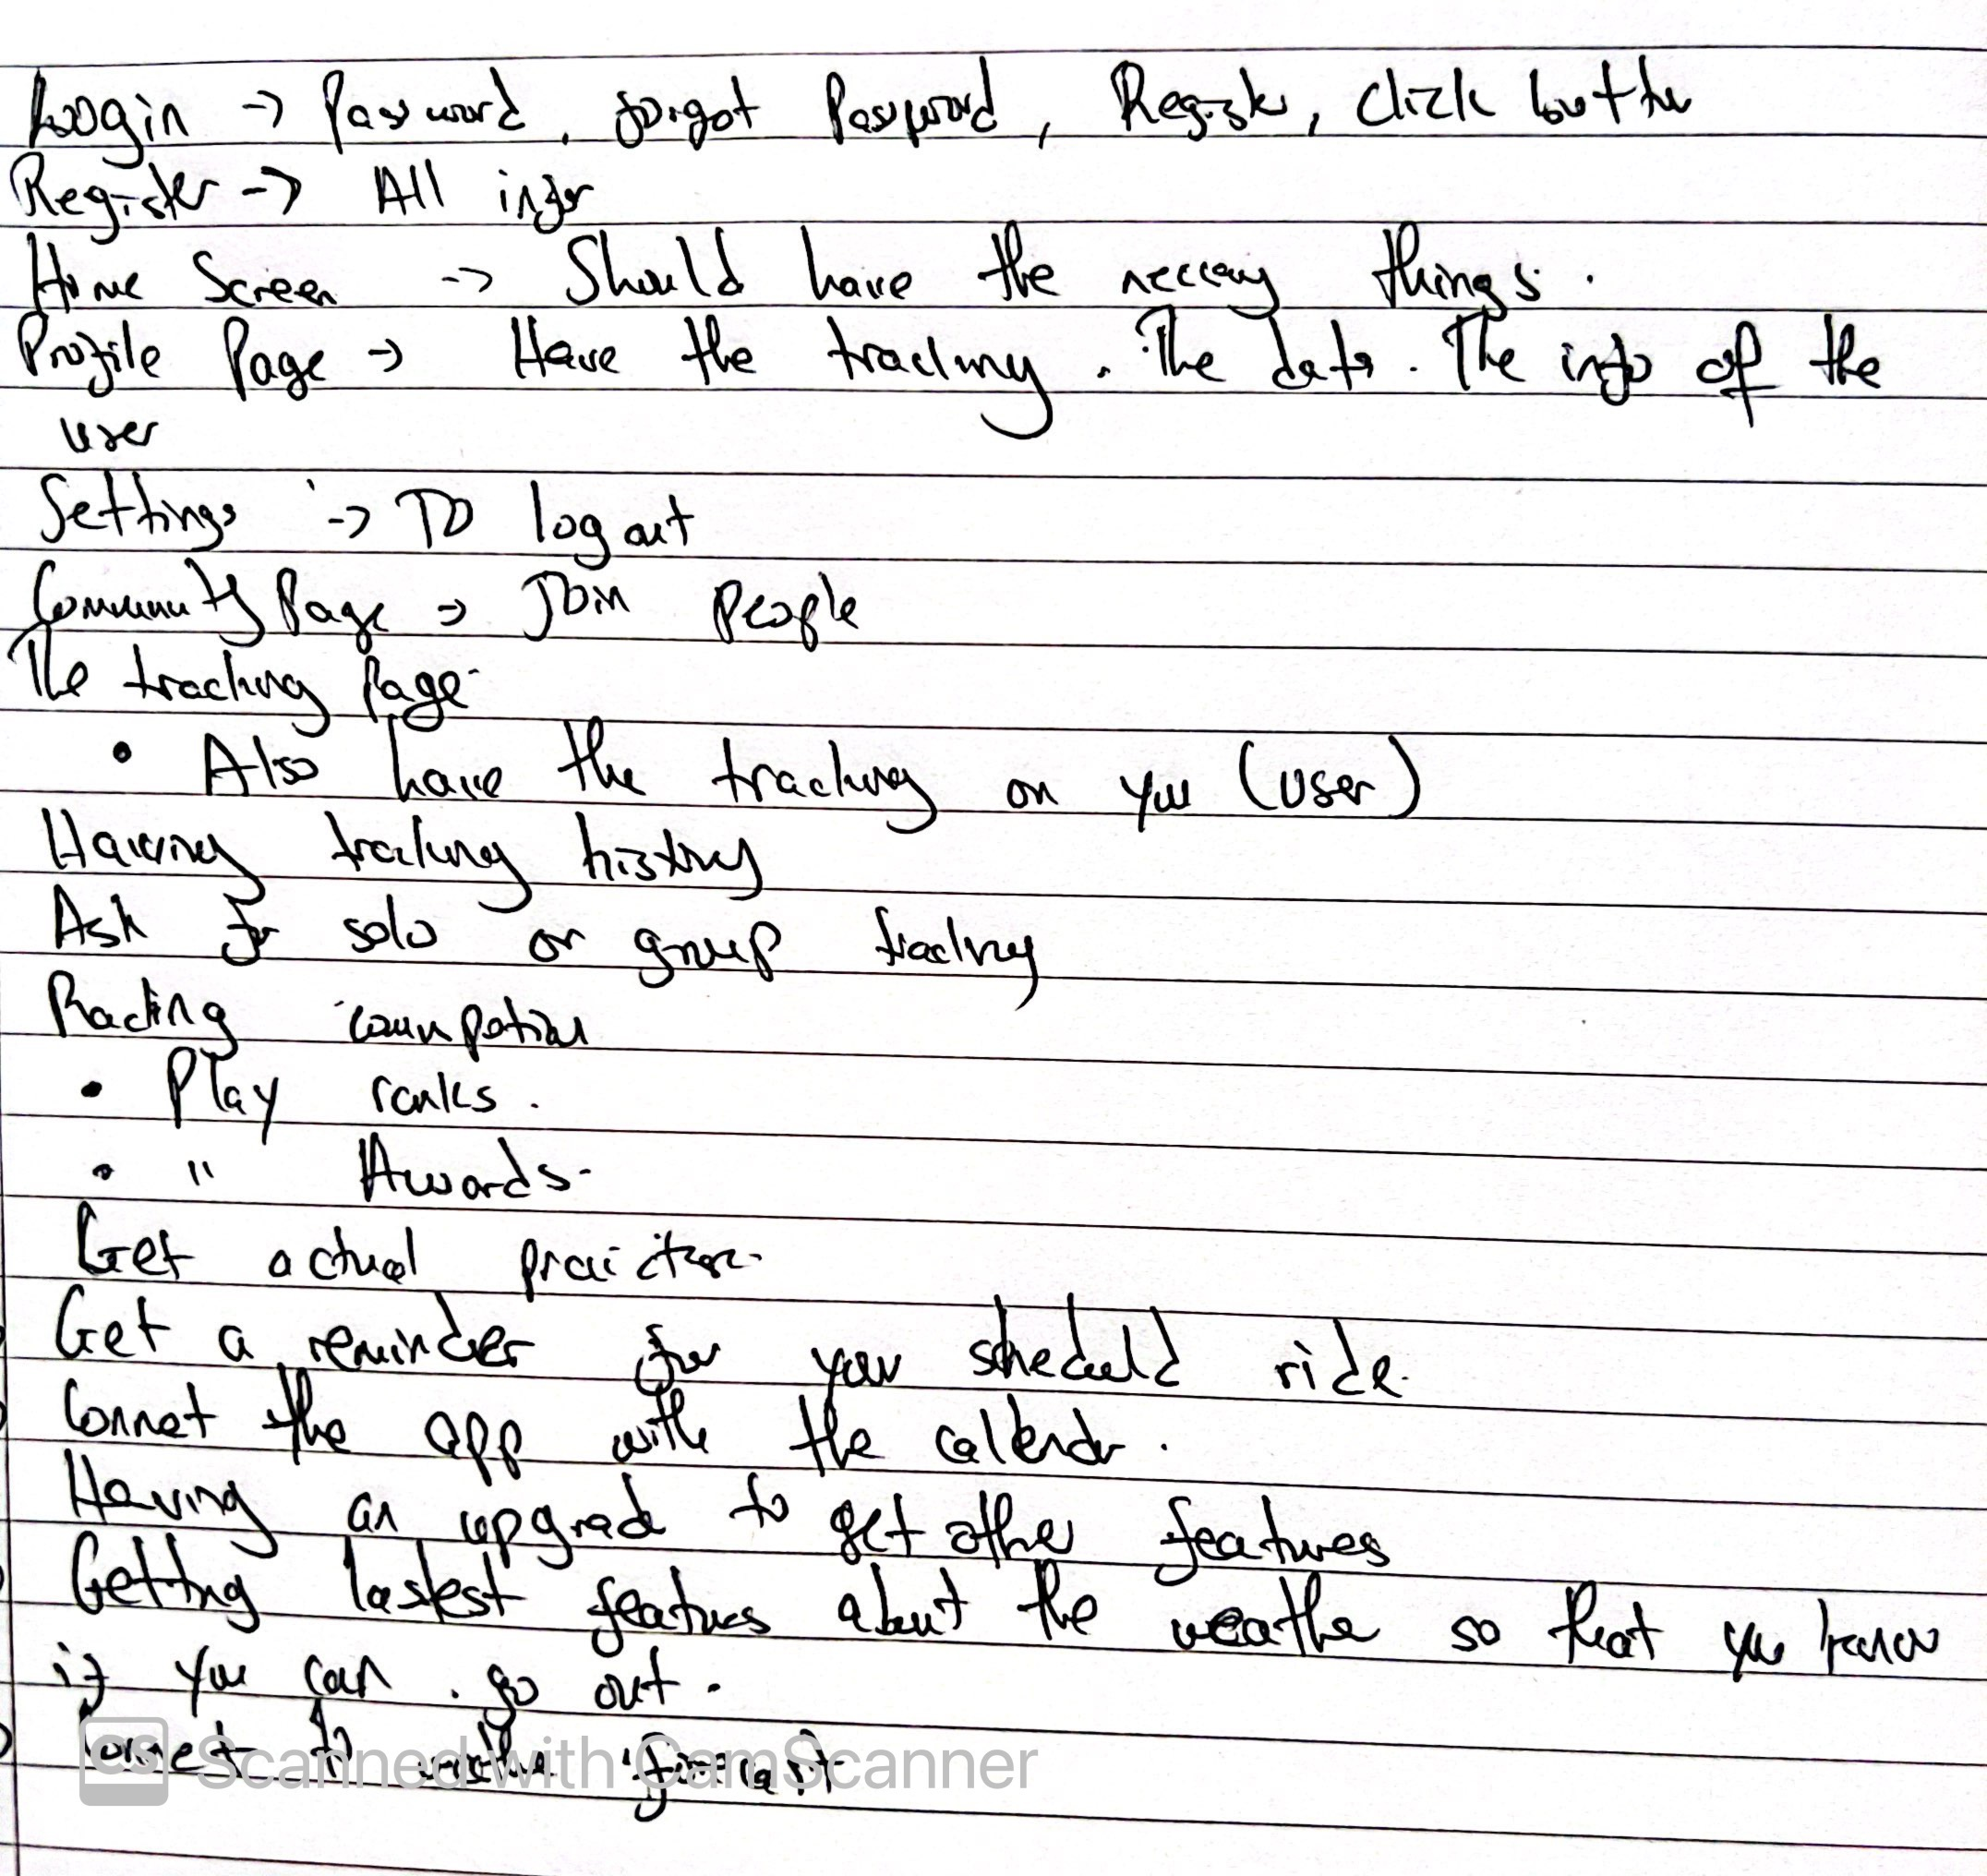
\includegraphics[width=1\textwidth]{images/think.JPG}
     \caption{think-aloud evaluation }
    \label{fig:Gettingideas}
\end{figure}


\subsection{Week 2}\label{UsabilityTestingWeekTwo}
Week 2 followed a similar structure to week 1, the new features were introduced then later explained to the participant's together with the expectations of the new week of testing. The second week ran smoothly. 
While adding in the features which was gathered from week one, then later testing it out to the participants. 
Unfortunately the user engagement, was much lower in the second week of testing compared to the first. This might  be because not all features was fully gathered. 



\section{Usability Evaluations - Late Stage}
The later stages of evaluation, such as the usability testing, consisted of high-fidelity prototypes, to evaluate these appropriately evaluation methods were introduced. As previously discussed, a survey was introduced at the end of the first week. The survey consisted of a number of closed and open-ended questions with goals to identify which features the participants were using the most,  which features had issues, and features the participants felt the application was lacking. The results and discussion of this survey can be seen in \textbf{Section \ref{resultssurvey}}.

At the end of the usability testing a semi-structured interview was run to gather further qualitative feedback. The interview consisted of questions to evaluate the usability, enjoyment and effectiveness of the application as a form of fitness tracking. The interviews are summarized and discussed in \textbf{Section \ref{Interviews}}.


\label{UsabilityEvaluationslaterstages}
\subsection{Survey}\label{resultssurvey}

The results of the survey suggested that the participants were already fairly active prior to using for the 1 week. 30\% of the participants also indicated that they were currently using a cycling app, with the tracker of choice listed as STRAVA. Three participants indicated they had stopped using the cycling app in the past due to a number of varying reasons, the main of which seemed to be the usability, with participants describing them as "hard to use" , "boring" or "not suit for them". 

The survey included questions on how easy was it to navigate the apps which shows that most of them found it easy to navigate the app. One of the participants made mention of how everything was clear and all icons where all common and easy to navigate.


Finally a host of open-ended questions were included, these were used to investigate more qualitative feedback. The feedback from these close ended-questions are On a scale of 1-10, please rate the overall design of the app (1 - very bad; 10 - very good),On a scale of 1-10, how much would you recommend the app to friends and family?, Did you find any of the pages particularly hard to navigate to/from?, If you answered "Yes" to the above, please tell us which page(s). If you answered "No", please tick "None of the above"., How easy was it to navigate the app. With an open ended question this as followers, Please list anything you would like to see improved...The feedback also indicated that some of the participants were finding the quests intangible. The quest distances were slightly shortened for week 2 after considering the feedback.

The feedback also confirmed the expected issues, users suggested that the search was unclear also the map page did not track or collect data. As it was not feasible to address this issue within the time scale, the users were prompted with another detailed explanation as to why the search functionality had been implemented with the code sharing implementation. 

 As the initial design decision was to stray away from a global leader board because it felt individualistic. The participants were also asked which other features they would most like to see in the application, with the following features being identified: 

\begin{itemize}
\item  More detailed main display (calorie information) 
\item Ability to view other progress
\item Leader board 
\end{itemize}


The interviews followed a semi-structured format to allow for follow-up questions in case the user raised aspects that weren't considered. The feedback from the interviews was relatively standard with most of the participants giving similar feedback, however a larger sample size and testing over longer periods would've resulted in more varied feedback.

The interviews started by asking the participants if they felt that were more active because of the application, with the majority of the participants feeling as though they were mildly more active. The participants that were already active and were averaging at least 5km a day felt no increase in activity while using the application. This may be down to the balancing between novice and veteran fitness users, as the participants who do not regularly engage in physical activity noted they felt "pressure" to contribute to the quests they were enrolled. The participants that mentioned they felt pressure to contribute considered it to be a positive consequence of the application.  

The next questions were regarding how and when the participants were using the application to obtain insight into the different scenarios of use. The uniform response here was that the participants were exploiting the background processing capabilities of the application, as users would make sure the app was at least open before starting their walk/run. Some participants noted that when their walk/run was over they would then open the application to check if the tracker had logged their distance. They stated that they also investigated the leader board features to check if their positions had changed. 

As a follow-up to how the participants were using the application post and pre-walks/runs they were asked which features they found themselves engaging with the most. One of the participants stated: "When the leader board was sort of introduced, I was kind of checking that quite a lot as well, because I think that was like a very fun element to it.". This appeared to be a consensus across the participants, which was confirmed when corroborated against the analytics in week 2 as the leader board was firmly in the top 3 views in terms of user engagement.

The next follow-up question presented to the participants was which feature they used the least and why? The uniform answer here was the battle feature, with all the participants linking the issues to the battle matchmaking functionality. One participant stated the following when asked why the battle feature was their least used: "Purely because of the way you have to sort of enter a game ID and stuff. So it just sort of slipped my mind a little bit because I knew that you have to like share the code and then just never got round to doing it.". 

The participants were asked if they would've engaged more with this feature had it not utilised the code sharing functionality. The overwhelming consensus was that the participants would've preferred the ability to directly send invites from within the application itself. One of the participants noted the following: "I think so, if I could invite someone directly through the app like I see this person and I can just click like invite.".

Finally the participants were asked about the new features introduced to the application. The consensus here was that the participants found the leader board very engaging, and added a form of friendly competition to the application. The participants also noted they found the new calorie feature informative, however stating that the calorie calculator would not remember their previously entered height and weight. 

Overall the interviews revealed which features had potential to inspire long term use, however they also revealed that the application lacked certain elements from the habit loops identified in \textbf{Section \ref{healthbehaviourchange}}. This was evident in the distance for the goals within the quests, as this required more thorough game balancing to achieve a challenging yet achievable goal distance. The overwhelming feedback from the interviews focused on the lack of engagement in the battles, as the participants were unfamiliar with each other it resulted in hesitancy to engage in the communication channels with one other.   






\chapter{Conclusion}   

\section{Summary}

The rise of multiple biking has prompted an abundance of research into the effectiveness of trackers for health behaviour change. The overwhelming conclusion is that the tracking of the app is not effective and needs to be improved.
 


As the aim was develop a bike tracking that tracks the steps of the bike , the time constraints of the project were not ideal. As the limited time meant that the usability testing would not be run over a long enough period of time the aims of the project were adjusted as follows: 

\begin{itemize}
    \item Research more issues of the modern bike trackers to identify potential solutions.
    \item Design and implement a bike tracker that incorporates collaborative features and  elements through an iterative design process. 
    \item Evaluate the potential of certain features and the application as a whole.
\end{itemize}

The project followed an iterative design process with the initial phases consisting mainly of concept generation and low-fidelity prototypes. As is the nature of iterative design processes early stage evaluations were run on the prototypes to identify the features and elements that had potential. The latter stages of the project consisted of software engineering practices in development of the iOS application. The final iteration entailed two weeks of usability testing, this was intertwined with evaluations such as surveys and interviews to gain qualitative feedback.

Quantitative feedback was gained during the usability testing by integrating two forms on analytics software. The first type was used to aggregate user interaction and generate heat maps, this allowed us to visualize the user interaction. The second type of analytics software recorded user events and the average amount of time spent on different views, this allowed us to investigate which views were most popular and how intensely the users were engaging in them. 

From the results of both the quantitative and qualitative feedback gained it is clear that the game elements as well as the collaborative features perform well in increasing engagement over a short period of time. The collaborative features were the most popular feature when corroborated against the data collected, it stands to reason that a multiplayer focused activity tracker that utilises game elements has the potential for long term behavioural change, however this can not be proven until run over a longer study. The activity tracker had the most substantial impact for novice bike users as they recorded they noticed increases in their activity during the study. 


\section{Future Work}


From the project and evaluation we have identified a number of avenues for future work, studies on collection of the data and the competition should be improved.

The more the sample size the better results will be. As of only having few participants and with the change of weather. Also, having professional participants will be a lot desirable. Participants  with past history of cycling as a racer or having a group of real professional cyclists will give more details on the testing. 

The evaluations also revealed features that due to limited time and development resources were not implemented, future work could look to implement and evaluate these features like collection of data, tracking of the user while on the phone. 

Also, adding more features like. 


- Connecting the app with weather forecast to detect when to ride or not due to the weather.


- Having an upgrade feature.


- Connecting the app with the calendar app. This will help set when the user will like to ride.


- Having a real live international race competition 


- Having a setting page.

- Having a countdown for the play button









%==================================================================================================================================
%
% 
%==================================================================================================================================
%  APPENDICES  

\begin{appendices}

\chapter{Usability evaluation - Survey} \label{appendixsurvey}

\begin{figure}[h!]
    \centering
    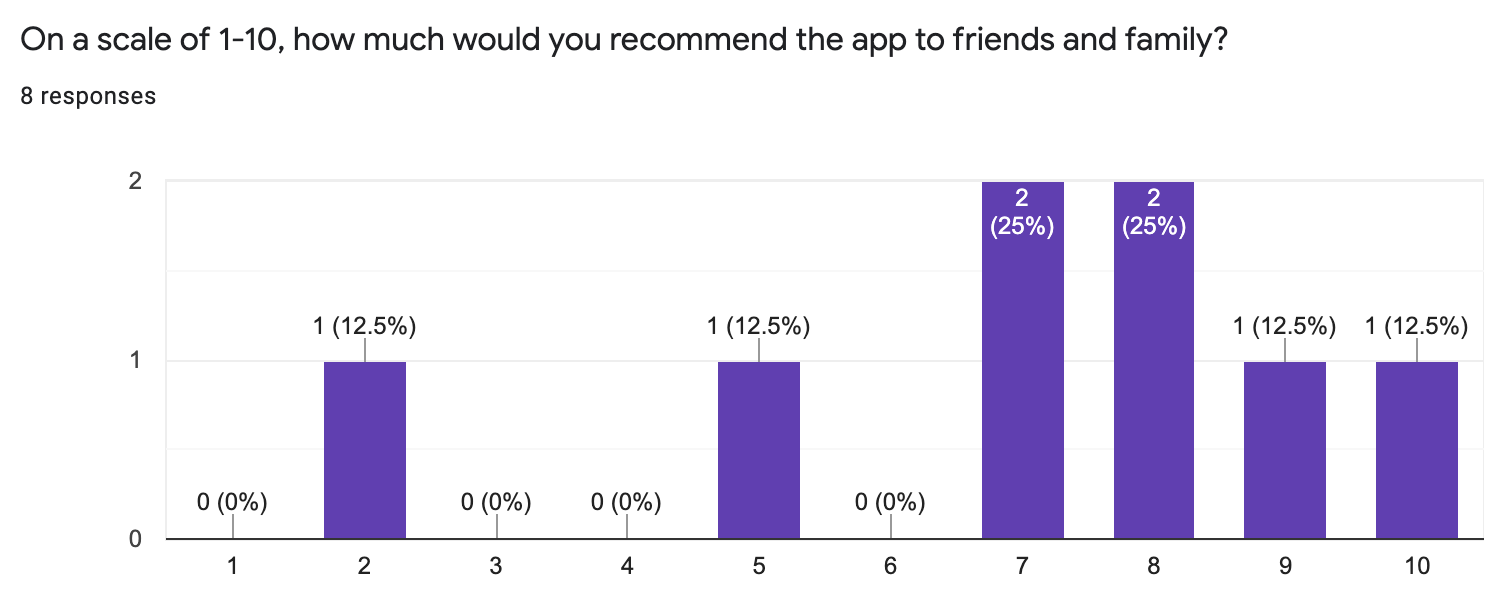
\includegraphics[scale=0.55]{images/Screenshot 2022-02-17 at 11.17.49 pm.png}
    \caption{Usability survey page one}
    \label{fig:surveypage1}
\end{figure}

\begin{figure}[h!]
    \centering
    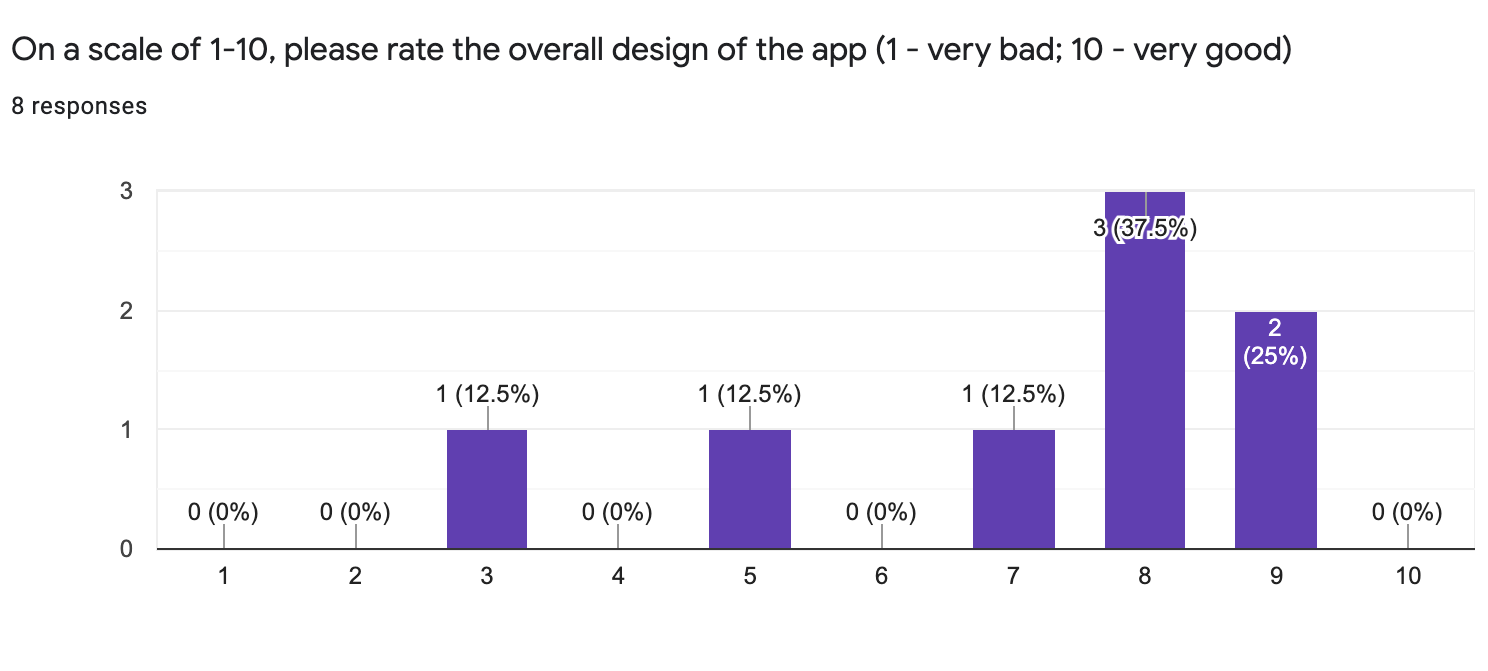
\includegraphics[scale=0.6]{images/Screenshot 2022-02-17 at 11.17.46 pm.png}
    \caption{Usability survey page two}
    \label{fig:surveypage2}
\end{figure}

\begin{figure}[h!]
    \centering
    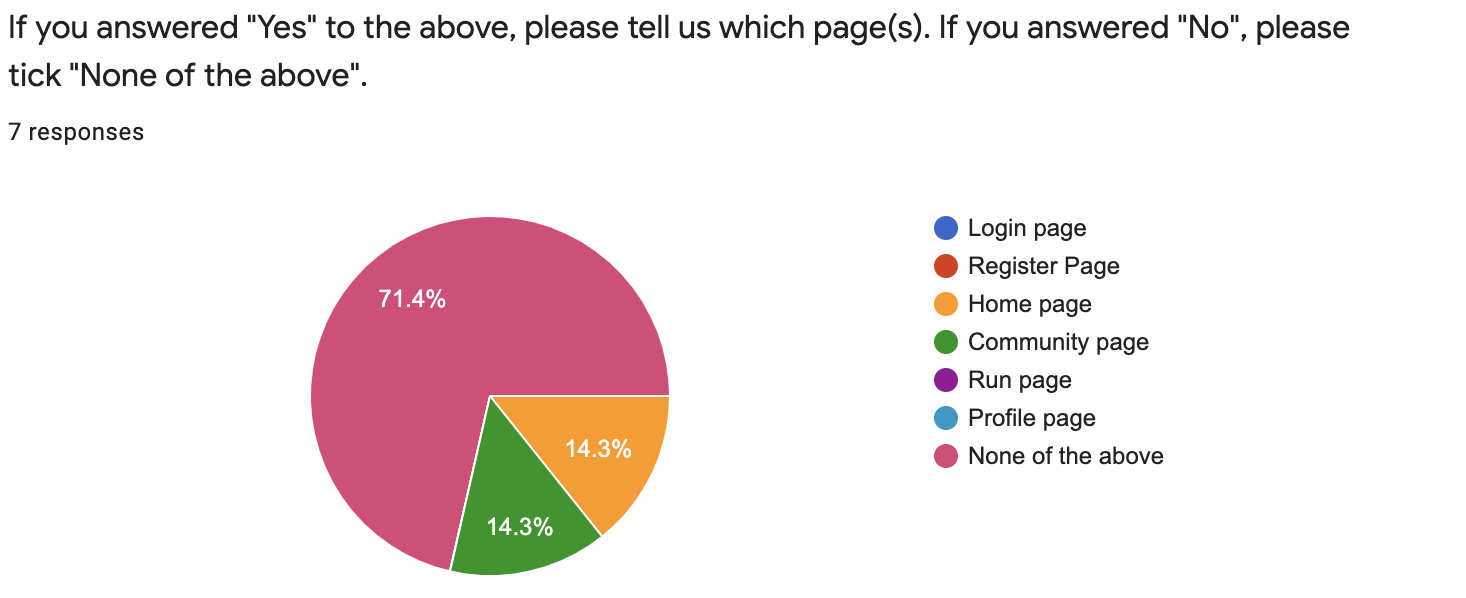
\includegraphics[scale=0.6]{images/Screenshot 2022-02-17 at 11.17.44 pm.png} 
    \caption{Usability survey page three}
    \label{fig:surveypage3}
\end{figure}

\begin{figure}[h!]
    \centering
    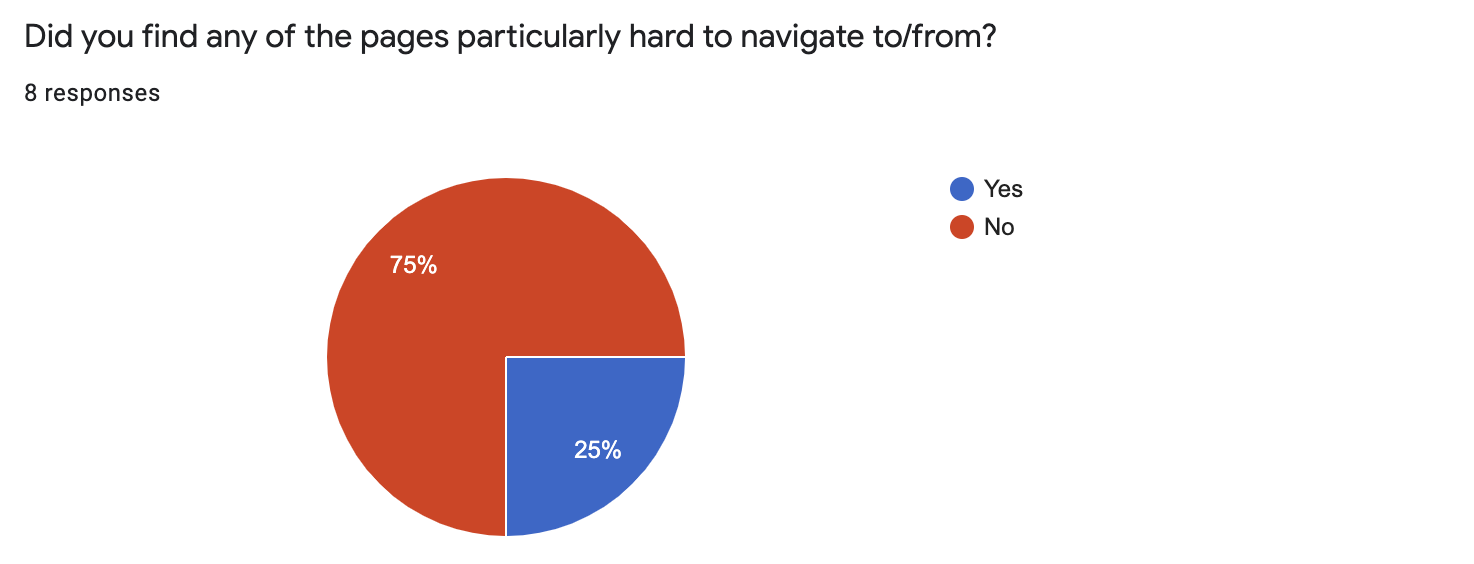
\includegraphics[scale=0.6]{images/Screenshot 2022-02-17 at 11.17.42 pm.png} 
    \caption{Usability survey page four}
    \label{fig:surveypage4}
\end{figure}

\begin{figure}[h!]
    \centering
    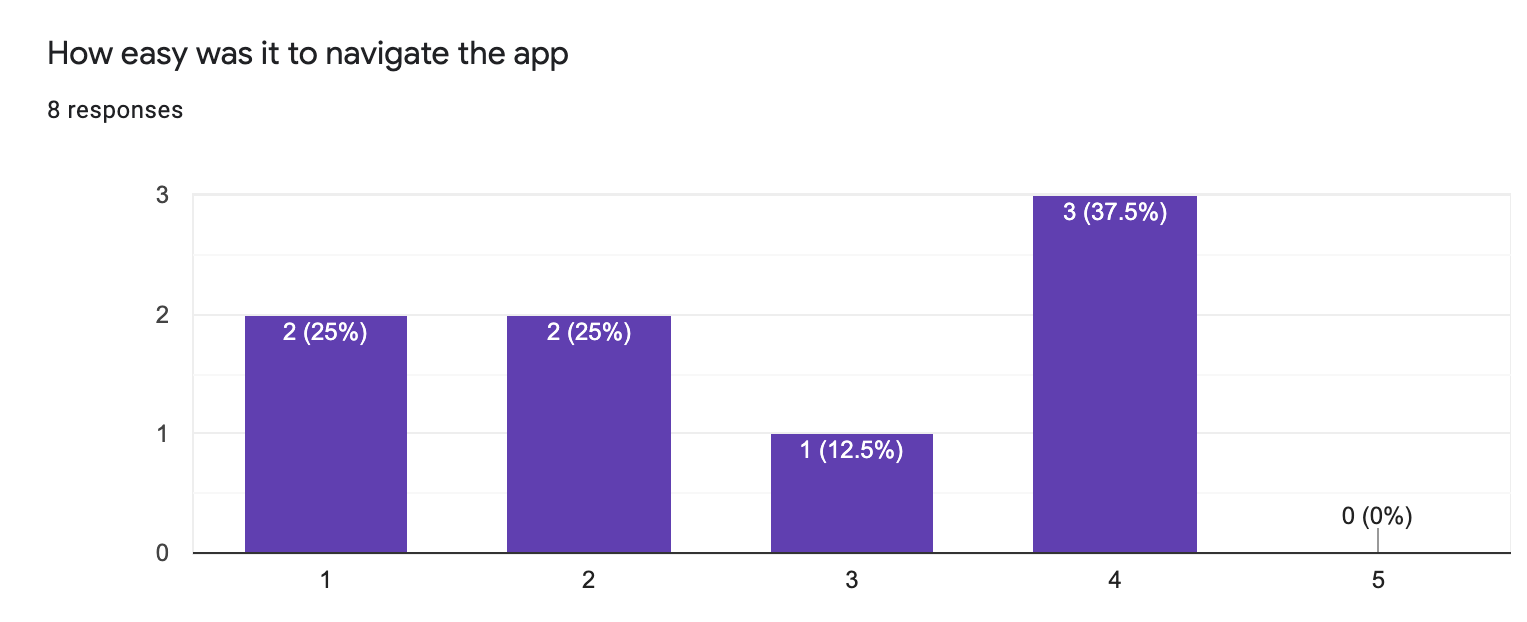
\includegraphics[scale=0.6]{images/Screenshot 2022-02-17 at 11.17.34 pm.png} 
    \caption{Usability survey page five}
    \label{fig:surveypage5}
\end{figure}

\begin{figure}[h!]
    \centering
    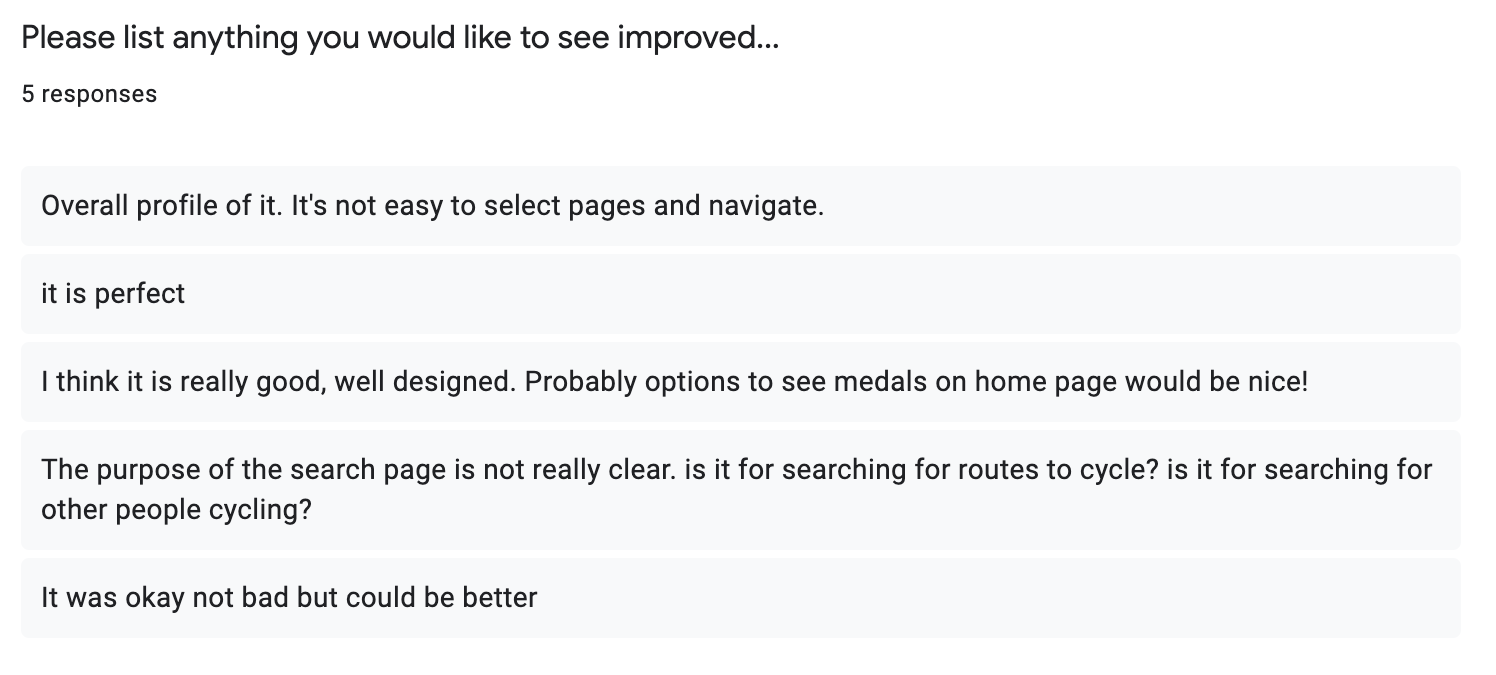
\includegraphics[scale=0.6]{images/Screenshot 2022-02-17 at 11.17.50 pm.png} 
    \caption{Usability survey page seven}
    \label{fig:surveypage7}
\end{figure}



\end{appendices}

%==================================================================================================================================
%   BIBLIOGRAPHY   

% The bibliography style is abbrvnat
% The bibliography always appears last, after the appendices.

\bibliographystyle{abbrvnat}

\bibliography{l4proj}

\end{document}